\documentclass[a4paper]{article}
\usepackage[english]{babel}
\usepackage[utf8]{vietnam}

%\usepackage{vntex}

%\usepackage[english,vietnam]{babel}
%\usepackage[utf8]{inputenc}

%\usepackage[utf8]{inputenc}
%\usepackage[francais]{babel}
\usepackage{a4wide,amssymb,epsfig,latexsym,multicol,array,hhline,fancyhdr}

\usepackage{amsmath}
\usepackage{lastpage}
\usepackage[lined,boxed,commentsnumbered]{algorithm2e}
\usepackage{enumerate}
\usepackage{color}
\usepackage{graphicx}
\usepackage{listings}
\lstset{frame=tb,
  language=C,
  aboveskip=3mm,
  belowskip=3mm,
  showstringspaces=false,
  columns=flexible,
  basicstyle={\small\ttfamily},
  numbers=none,
  numberstyle=\tiny\color{gray},
  keywordstyle=\color{blue},
  commentstyle=\color{dkgreen},
  stringstyle=\color{mauve},
  breaklines=true,
  breakatwhitespace=true,
  tabsize=3
}
\definecolor{dkgreen}{rgb}{0,0.6,0}
\definecolor{gray}{rgb}{0.5,0.5,0.5}
\definecolor{mauve}{rgb}{0.58,0,0.82}
% Standard graphics package
\usepackage{array}
\usepackage{tabularx, caption}
\usepackage{multirow}
\usepackage{multicol}
\usepackage{rotating}
\usepackage{graphics}
\usepackage[a4paper,left=2cm,right=2cm,top=1.8cm,bottom=2.8cm]{geometry}
\usepackage{setspace}
\usepackage{epsfig}
\usepackage{tikz}
\usetikzlibrary{arrows,snakes,backgrounds}
\usepackage[unicode]{hyperref}
%can file puenc.def trong thu muc goc de option [unicode] tao ra bookmark bang tieng Viet
\hypersetup{urlcolor=blue,linkcolor=black,citecolor=black,colorlinks=true} 
%\usepackage{pstcol} 								
% PSTricks with the standard color package

\newtheorem{theorem}{{\bf Theorem}}
\newtheorem{property}{{\bf Property}}
\newtheorem{proposition}{{\bf Proposition}}
\newtheorem{corollary}[proposition]{{\bf Corollary}}
\newtheorem{lemma}[proposition]{{\bf Lemma}}


%\usepackage{fancyhdr}
\setlength{\headheight}{40pt}
\pagestyle{fancy}
\fancyhead{} % clear all header fields
\fancyhead[L]{
 \begin{tabular}{rl}
    \begin{picture}(25,15)(0,0)
    \put(0,-8){
\includegraphics[width=8mm, height=8mm]{hcmut.png}}
    %\put(0,-8){\epsfig{width=10mm,figure=hcmut.eps}}
   \end{picture}&
	%
\includegraphics[width=8mm, height=8mm]{hcmut.png} & %
	\begin{tabular}{l}
		\textbf{\bf \ttfamily Ho Chi Minh City University of Technology, VNU-HCM}\\
		\textbf{\bf \ttfamily Faculty of Electrical \&  Electronics Engineering}
	\end{tabular} 	
 \end{tabular}
}
\fancyhead[R]{
	\begin{tabular}{l}
		\tiny \bf \\
		\tiny \bf 
	\end{tabular}  }
\fancyfoot{} % clear all footer fields
\fancyfoot[L]{\scriptsize \ttfamily Report - Embedded System Design, 2020}
\fancyfoot[R]{\scriptsize \ttfamily Page {\thepage}/\pageref{LastPage}}
\renewcommand{\headrulewidth}{0.3pt}
\renewcommand{\footrulewidth}{0.3pt}
\setcounter{secnumdepth}{4}
\setcounter{tocdepth}{3}

%%%

\makeatletter
\newcounter {subsubsubsection}[subsubsection]
\renewcommand\thesubsubsubsection{\thesubsubsection .\@alph\c@subsubsubsection}
\newcommand\subsubsubsection{\@startsection{subsubsubsection}{4}{\z@}%
                                     {-3.25ex\@plus -1ex \@minus -.2ex}%
                                     {1.5ex \@plus .2ex}%
                                     {\normalfont\normalsize\bfseries}}
\newcommand*\l@subsubsubsection{\@dottedtocline{3}{10.0em}{4.1em}}
\newcommand*{\subsubsubsectionmark}[1]{}
\makeatother


\begin{document}

\begin{titlepage}

\begin{center}
HO CHI MINH CITY UNIVERSITY OF TECHNOLOGY, VNU-HCM\\
FACULTY OF ELECTRICAL \& ELECTRONICS ENGINEERING
\end{center}

\vspace{1cm}

\begin{figure}[h!]
\begin{center}

\includegraphics[width=3cm]{hcmut.png}
\end{center}
\end{figure}

\vspace{1cm}


\begin{center}
\begin{tabular}{c}
\multicolumn{1}{l}{\textbf{{\Large EMBEDDED SYSTEM DESIGN}}}\\
~~\\
\hline
\\
\multicolumn{1}{l}{\textbf{{\Large Report}}}\\
\\
\textbf{\Huge DTMF remote control appliances}\\
\\
\hline
\end{tabular}
\end{center}

\vspace{3cm}

\begin{table}[h]
\begin{tabular}{rrl}

\hspace{5 cm} & Tutor: Trần Hoàng Quân & (thquan@hcmut.edu.vn)\\
& Class: A02\\
& Student members: & Nguyễn Thành Trung - 1814515 \\
& & Phan Nguyên Trung - 1814519 \\
& & Hoàng Đình Toản - 1814379 \\
& & Trương Văn Sáng - 1813825 \\

\end{tabular}
\end{table}

\begin{center}
{\footnotesize Ho Chi Minh, 11/2019}
\end{center}
\end{titlepage}


%\thispagestyle{empty}
\selectlanguage{english}
\begin{center}
\huge
\textbf{Acknowledgements}
\end{center}
Today, with the applications of advanced science and technology, our world has been changing, civilized and more modern day by day. The development of electronic engineering has created a series of devices with outstanding features such as high precision, fast speed, and compactness that are essential factors contributing to human operation to be effective.\\
Electronics is becoming a multitasking science. It has met the essential needs in daily life. One of those needs is remote control.\\
In addition, due to the need to apply the knowledge we learned at class into life, we have chosen the topic "DTMF remote control appliances" to do a project in the subject.\\
After a period of study and practice, with the devoted guidance of teacher Mr. Tran Quan, we have had the project completed.\\
Many shortcomings cannot be avoided, we hope Mr. Tran understand and instruct more so that the topic can be widely applied in practice.
\newpage
\vspace*{\fill}
{\centering This page would be intentionally left blank if we would not wish to inform about that.\par}
\vspace{\fill}
\newpage
\tableofcontents
\newpage
\vspace*{\fill}
{\centering This page would be intentionally left blank if we would not wish to inform about that.\par}
\vspace{\fill}
\newpage
%%%%%%%%%%%%%%%%%%%%%%%%%%%%%%%%%
\section{Introduction}
\label{introduction}
\subsection{Overview}
In the modern day, smart homes will soon be available everywhere in the world which will allow its users to control and monitor their homes with a single application. However, these applications usually go along with a high cost and a strong internet connection which is not suitable for everyone. Therefore, we come with another solution that helps our users to control their appliances without using any internet connection. Also, the cost of this application will also be cheaper than other available solutions.\\
Our solution is DTMF (Dual-Tone Multi-Frequency) remote control via mobile phone, which is an application specific that can be used for controlling various appliances in a building or at home.\\
This DTMF extension is a universal module that can be connected to any microcontroller platform. It detects DTMF tones and decodes them to binary digits that can be easily read by microcontroller, which will decide what tasks to perform.\\
The system uses \textbf{Atmel AT89S52} microcontroller without external memory. Program is developed using Embedded C and compiled by KeilC.
\subsection{Features}
To give a user the usable and friendly system, we shall provide the following features:
\begin{itemize}
    \item To build a safety electrical appliances.
    \item Providing an user interface with friendly user experience.
    \item Allow user to get the timer for frequency tasks with variant options of time.
    \item Including a security system which easy to use with strong and changeable password.
    \item Also, the system has multiple options to control appliances with easy including DTMF and Manual control.
\end{itemize}
\subsection{Assignment}
The responsibilities of each member is shown in table below.
\begin{table}[h!]
\centering
\begin{tabular}{||c | c ||}
\hline
Name               & Role             \\ \hline
Hoàng Đình Toản \& Nguyễn Thành Trung & Develop software \\ \hline
Hoàng Đình Toản    & Develop hardware \\ \hline
Nguyễn Thành Trung \& Phan Nguyên Trung  & Test             \\ \hline
Trương Văn Sáng \& Phan Nguyên Trung    & Report           \\ \hline
\end{tabular}
\end{table}

\newpage
%%%%%%%%%%%%%%%%%%%%%%%%%%%%%%%%%
\section{System specification}\label{fornul}

\subsection{Product specification}
The primary function of the system is to control appliances via mobile phone that transmits DTMF signals. We can use keypad on the system also for convenience if we're not far from it.\\
The status of appliances, date and time will be displayed in a LCD screen help user to interact with. There will be a keypad for manual control as mentioned above.\\
The real world I/O consists of DTMF decoder, real-time clock, triacs and buzzer. There's no external interface.
\subsection{Hardware specification}
We will give you a quick overview of the system by modeling our system graphically and show the relationships in the process in the block diagram below.
\begin{figure}[h!]
\centering
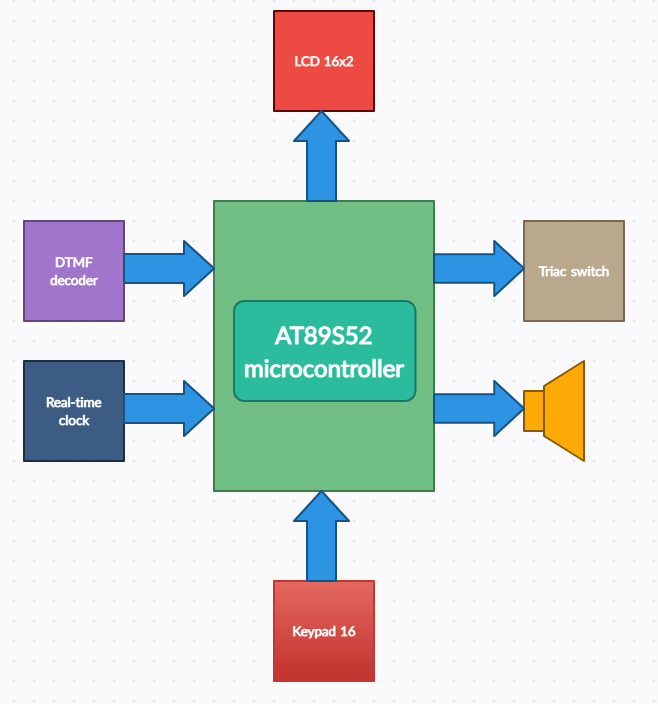
\includegraphics[width=15cm]{images/block_diagram.PNG}
\caption*{Block diagram}
\end{figure}
\subsubsection{Atmel AT89S52 microcontroller}
The AT89S52 is a low-power, high-performance CMOS 8-bit microcontroller with 8K
bytes of in-system programmable Flash memory. The device is manufactured using
Atmel’s high-density nonvolatile memory technology and is compatible with the industry-standard 80C51 instruction set and pinout. The on-chip Flash allows the program
memory to be reprogrammed in-system or by a conventional nonvolatile memory programmer. By combining a versatile 8-bit CPU with in-system programmable Flash on
a monolithic chip, the Atmel AT89S52 is a powerful microcontroller which provides a
highly-flexible and cost-effective solution to many embedded control applications.
\begin{figure}[h!]
\centering
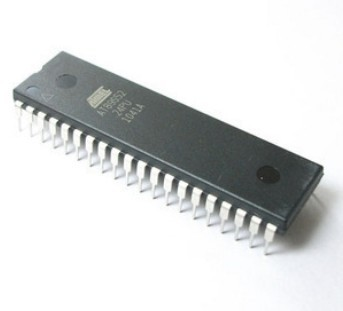
\includegraphics[width=6cm]{images/atmel_at89s52_microcontroller.jpg}
\caption*{Atmel AT89S52 microcontroller}
\end{figure}
\newline
\noindent
The AT89S52 provides the following standard features: 8K bytes of Flash, 256 bytes
of RAM, 32 I/O lines, Watchdog timer, two data pointers, three 16-bit timer/counters, a
six-vector two-level interrupt architecture, a full duplex serial port, on-chip oscillator,
and clock circuitry. In addition, the AT89S52 is designed with static logic for operation
down to zero frequency and supports two software selectable power saving modes.
The Idle Mode stops the CPU while allowing the RAM, timer/counters, serial port, and
interrupt system to continue functioning. The Power-down mode saves the RAM contents but freezes the oscillator, disabling all other chip functions until the next interrupt or hardware reset.
\begin{figure}[h!]
\centering
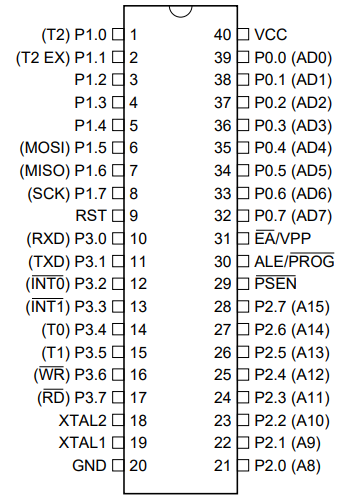
\includegraphics[width=6cm]{images/atmel_pins.PNG}
\caption*{Pin configuration}
\end{figure}

\subsubsection{Keypad 16}
Keypad 16 that is also known as keypad 4x4 is used for many kind of applications. Few are for easy to use input device is needed, input module can only have few pins or just professional look.
\begin{figure}[h!]
\centering
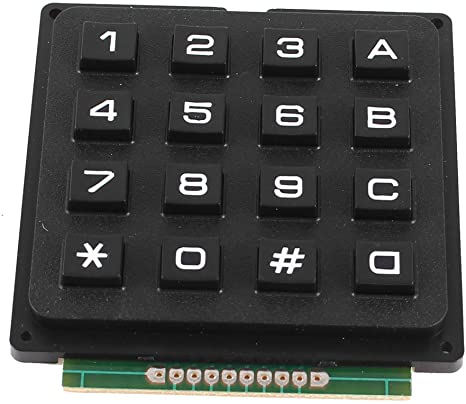
\includegraphics[width=6cm]{images/keypad.jpg}
\caption*{Keypad 16}
\end{figure}
\newline
\noindent
Using this module is little tricky. As 16 keys are connected in matrix formation the module is a little complex to use. The module gives only 8 pins as a way for interacting with 16 buttons.\\
We first set all rows to output and set them at +5V. Next set all columns as input to sense the high logic. Now consider a button is pressed on keypad. And that key is at 2nd column and 3rd row as below.\\
With the button being pressed the current flows as shown in figure. With that a voltage of +5V appears at terminal C2 (2nd column). Since the column pins are set as inputs, the controller can sense C2 going high. The controller can be programmed to remember that C2 going high and the button pressed is in C2 column.
\begin{figure}[h!]
\centering
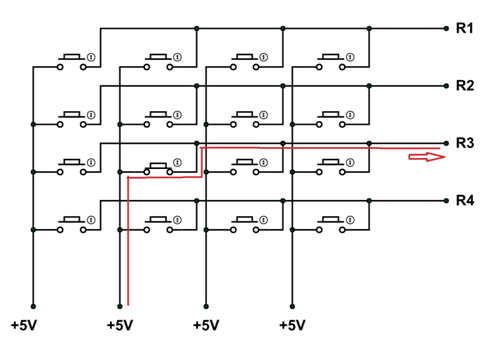
\includegraphics[width=9cm]{images/keypad_pins.png}
\caption*{Internal structure}
\end{figure}
\newline
\noindent
Next set all columns to output and set them at +5V. Next set all rows as input to sense the high logic. Since the key pressed is at 2nd column and 3rd row. The current flows as shown above.\\
With that current flow a positive voltage of +5V appears at R3 (3rd row) pin. Since all rows are set as inputs, the controller can sense +5V at R3 pin. The controller can be programmed to remember the key being pressed at third row.\\
From previous step, we have known the column number of key pressed and now we know row number. With that we can match the key being pressed. Therefore, we can take the key input provided by this way for keypad 16 module.

\subsubsection{MT8870 DTMF decoder}
The MT8870D/MT8870D-1 is a complete DTMF receiver integrating both the bandsplit filter and digital decoder functions. The filter section uses switched capacitor techniques for high and low group filters; the decoder uses digital counting techniques to detect and decode all 16 DTMF tone-pairs into a 4-bit code.\\
The MT8870 monolithic DTMF receiver offers small size, low power consumption and high
performance. Its architecture consists of a bandsplit filter section, which separates the high and low group tones, followed by a digital counting section which verifies the frequency and duration of the received tones before passing the corresponding code to the output bus. 

\begin{figure}[h!]
\centering
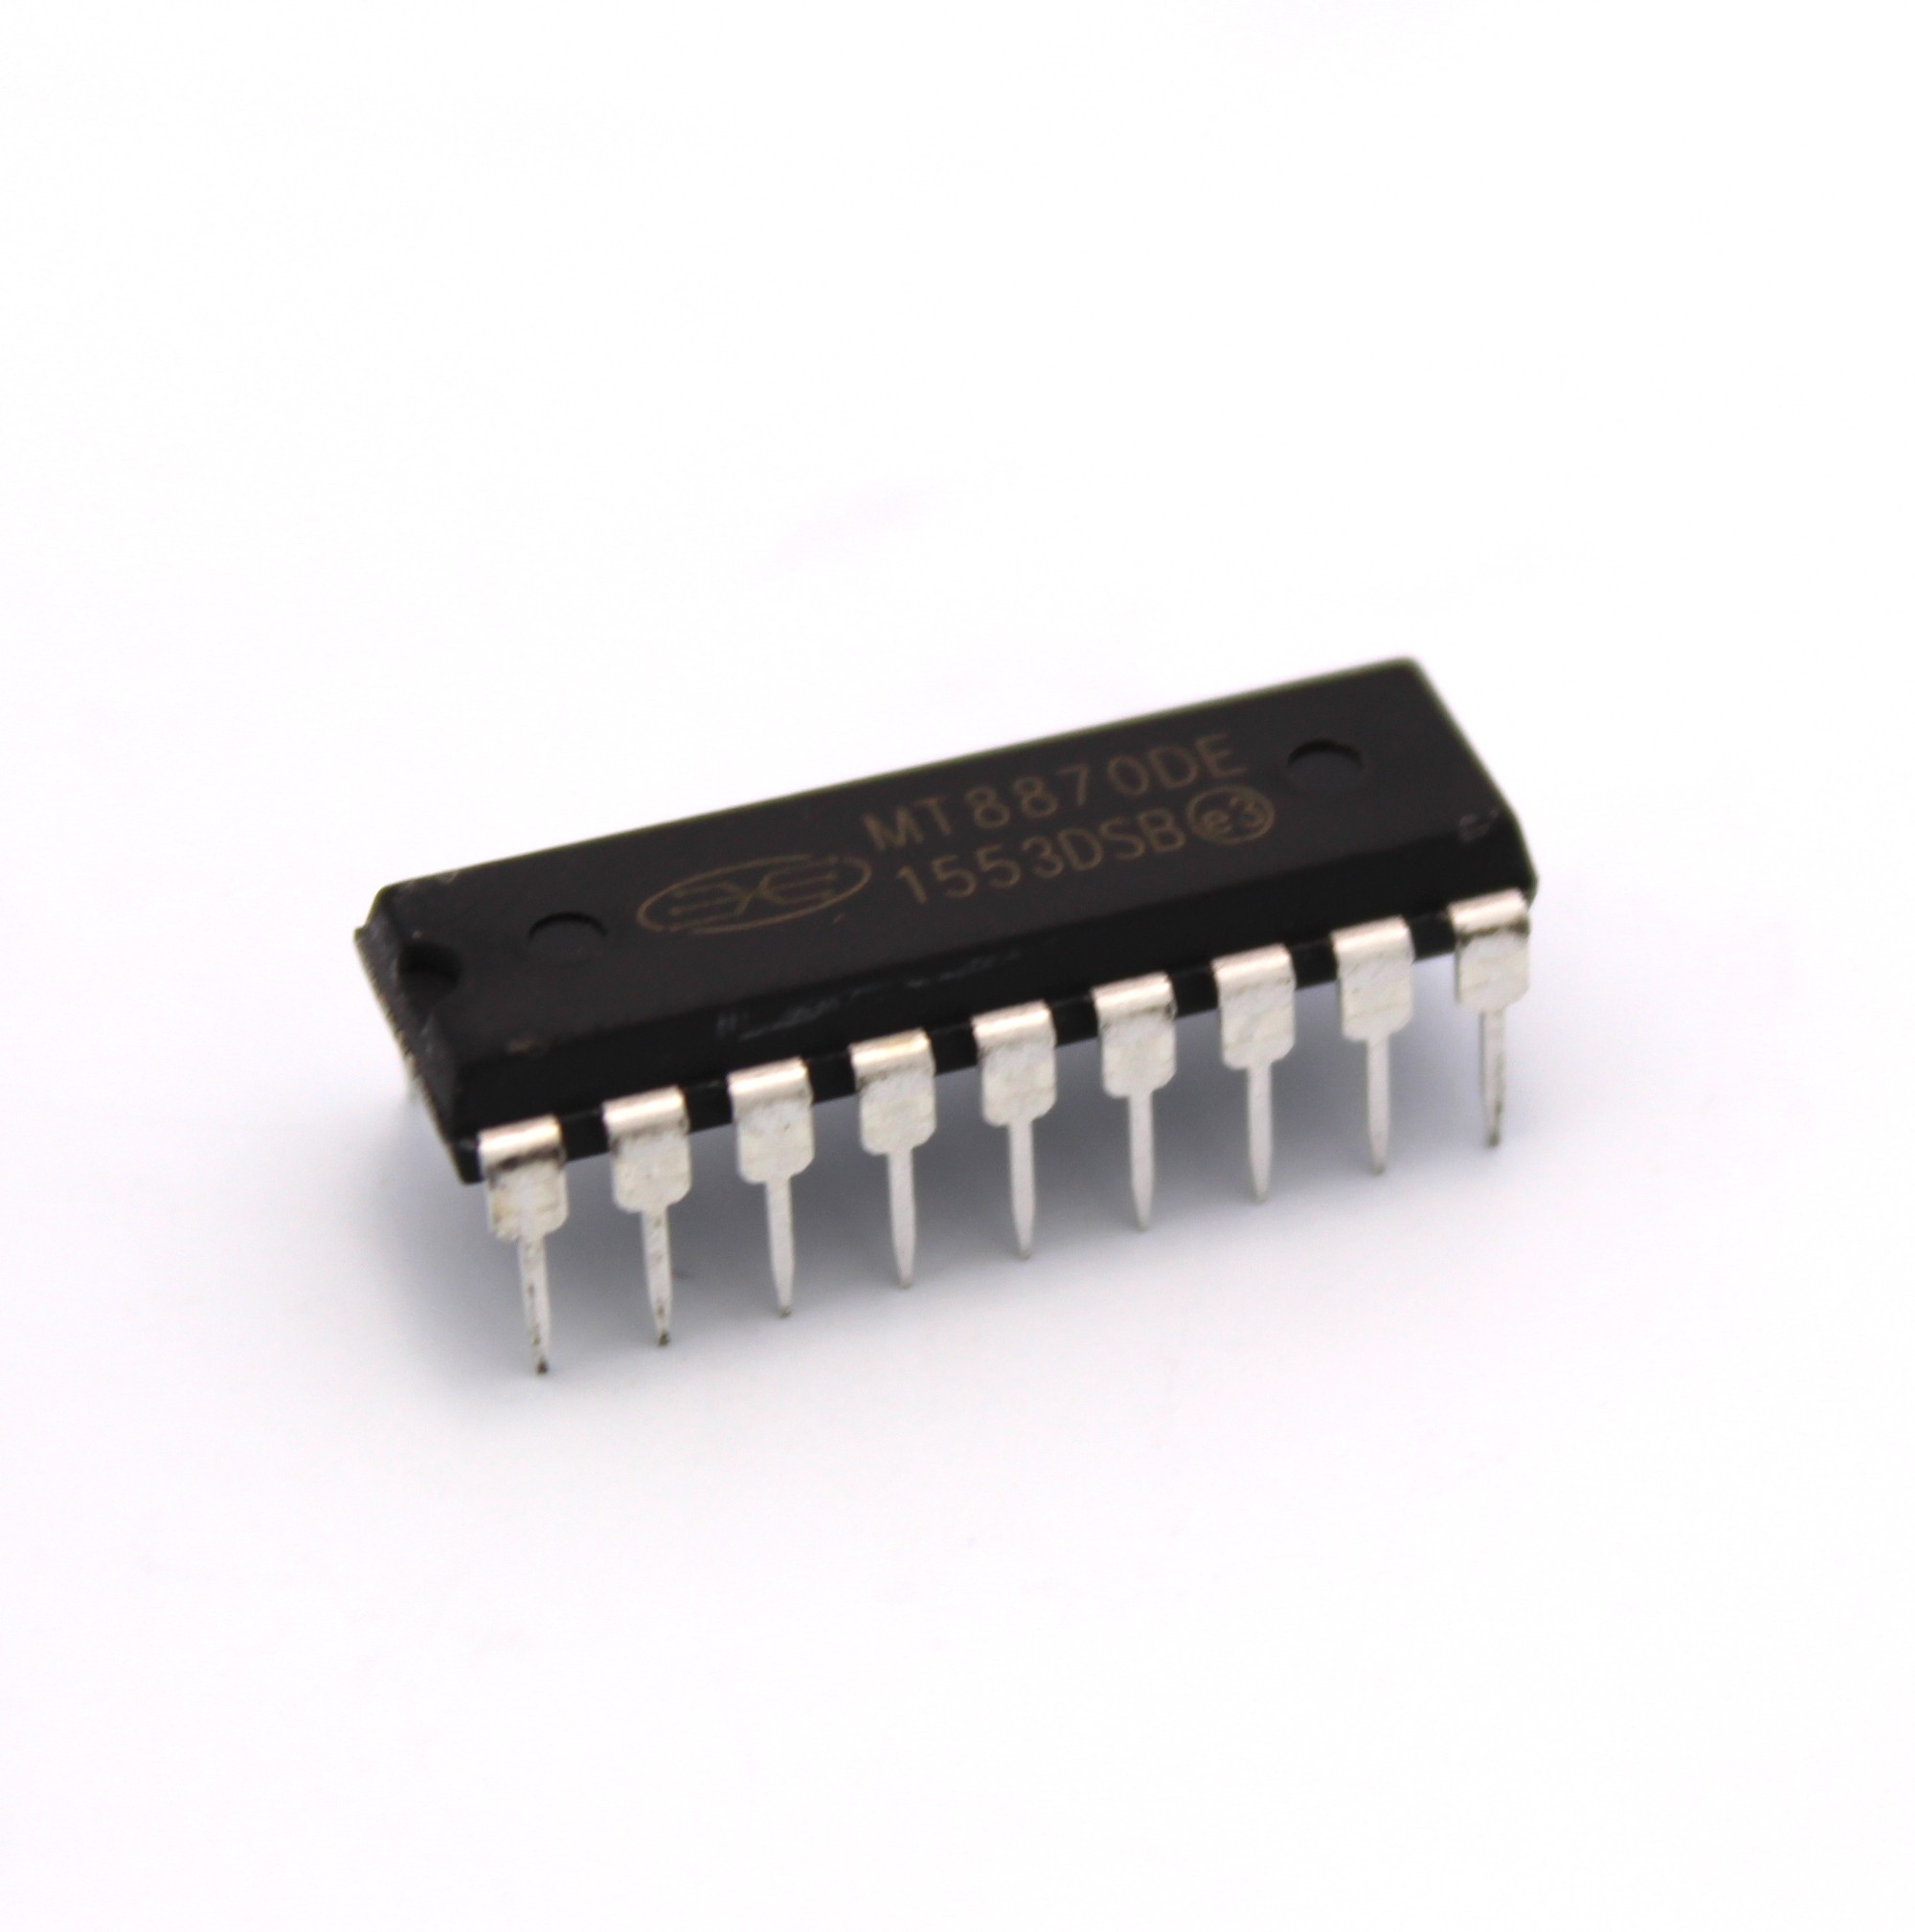
\includegraphics[width=6cm]{images/dtmf_decoder.jpg}
\caption*{MT8870 DTMF decoder}
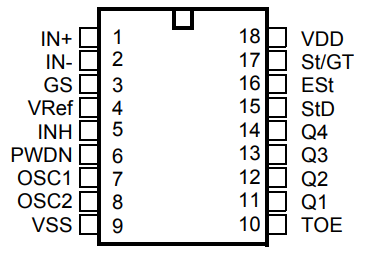
\includegraphics[width=8cm]{images/decoder_pins.PNG}
\caption*{Pin configuration}
\end{figure}
\newpage
\noindent
Further clarification on how this decoder work is beyond of the scope of this report but you can find it on \href{https://www.microsemi.com/document-portal/doc_view/127041-mt8870d-datasheet-oct2006}{MT8870D Data Sheet}

\subsubsection{Real-time clock DS1307}
The DS1307 serial real-time clock (RTC) is a lowpower, full binary-coded decimal (BCD) clock/calendar plus 56 bytes of NV SRAM. Address and data are transferred serially through an I2C, bidirectional bus. The clock/calendar provides seconds, minutes, hours, day, date, month, and year information. The end of the month date is automatically adjusted for months with fewer than 31 days, including corrections for leap year. The clock operates in either the 24-hour or 12-hour format with AM/PM indicator. The DS1307 has a built-in power-sense circuit that detects power failures
and automatically switches to the backup supply. Timekeeping operation continues while the part operates from the backup supply.
\begin{figure}[h!]
\centering
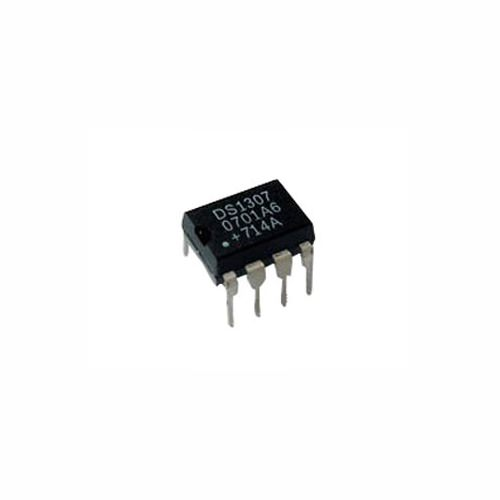
\includegraphics[width=5.13cm]{images/dsa.jpg}
\caption*{Real-time clock DS1307}
\end{figure}
\begin{figure}[h!]
\centering
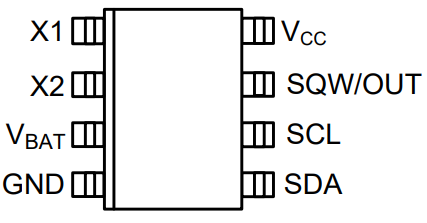
\includegraphics[width=8cm]{images/dsa_pins.PNG}
\caption*{Pin configuration}
\end{figure}
\newline
\noindent
Benefits and features made us to use the DS1307 are:
 \begin{itemize}
   \item  Completely Manages All Timekeeping Functions
   \begin{itemize}
     \item  Real-time clock counts seconds, minutes, hours, date of the month, month, day of the week, and year with leap-year compensation valid pp to 2100.
     \item 56-byte, battery-backed, general-purpose RAM with unlimited writes.
     \item Programmable square-wave output signal.
   \end{itemize}
   \item Simple serial port interfaces to most microcontrollers
   \begin{itemize}
       \item $\mathrm{I^2C}$ serial interface.
   \end{itemize}
   \item Low power operation extends battery backup run time
   \begin{itemize}
       \item Consumes less than 500nA in battery backup mode with oscillator running.
       \item Automatic power-fail detect and switch circuitry.
   \end{itemize}
   \item 8-Pin DIP and 8-Pin SO minimizes required space
   \item Optional industrial temperature range: -40°C to +85°C supports operation in a wide range of applications
 \end{itemize}

\subsubsection{LCD 16x2}
A 16x2 LCD display is very basic module and is very commonly used in various devices and circuits. It can display 16 characters per line and there are 2 such lines. In this LCD, each character is displayed in 5x7 pixel matrix. The 16 x 2 intelligent alphanumeric dot matrix display is capable of displaying 224 different characters and symbols.
\begin{figure}[h!]
\centering
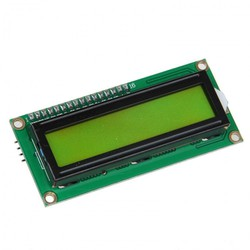
\includegraphics[width=7.55cm]{images/lcd.jpg}
\caption*{LCD 16x2}
\end{figure}

\subsubsection{Optocoupler triac MOC3021 \& Triac BTA12}
The MOC3021 is optically isolated triac driver devices. This device contains a GaAs infrared emitting diode and a light activated silicon bilateral switch, which functions like a triac. It is designed for interfacing between electronic controls and power triacs.
\begin{figure}[h!]
\centering
{{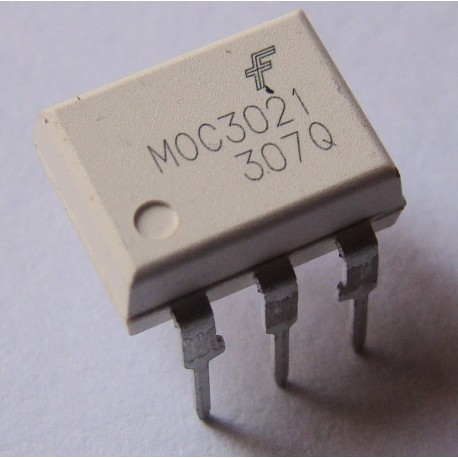
\includegraphics[width=6cm]{images/moc_triac.jpg} }}
\qquad
{{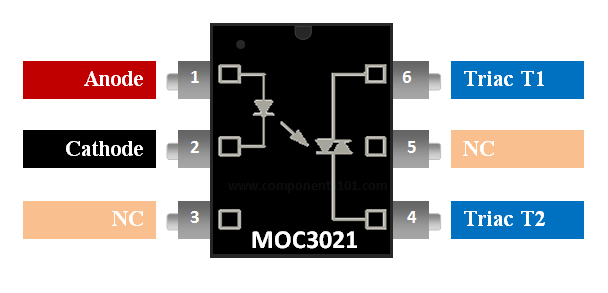
\includegraphics[width=10cm]{images/mocpin.png} }}
\caption*{Optocoupler triac MOC3021 and pin configuration}
\end{figure}
\newline
\noindent
For BTA12, this triac can be used as ON/OFF function in applications such as static relays, heating regulation or induction motor starting circuit. It is also recommended for phase control operations in light dimmers and appliance motors speed controllers.\\
Logic Level BTA12 offer low holding current, ideal to design light dimmers for LED lamps.
\begin{figure}[h!]
\centering
{{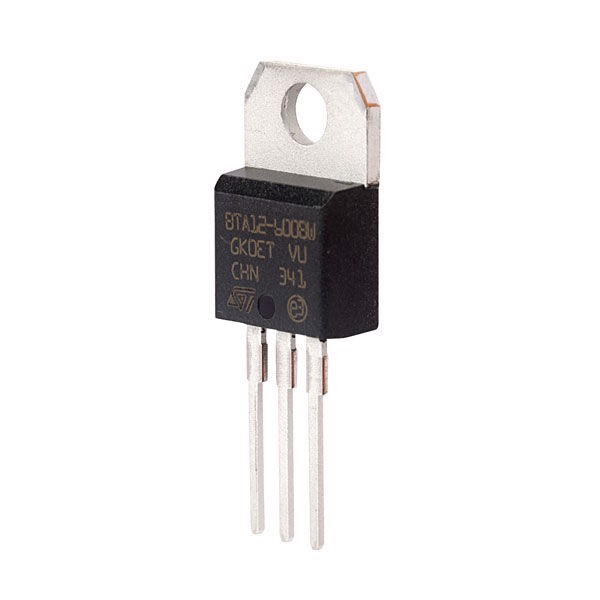
\includegraphics[width=6cm]{images/bta_triac.jpg} }}
\qquad
{{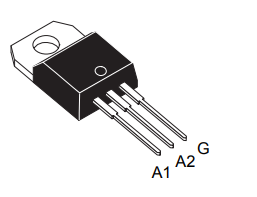
\includegraphics[width=8cm]{images/btapin.PNG} }}
\caption*{Triac BTA12 and pin configuration}
\end{figure}
\subsubsection{Buzzer 5V}
A buzzer or beeper is an audio signaling device, which may be mechanical, electromechanical, or piezoelectric. Typical uses of buzzers and beepers include alarm devices, timers and confirmation of user input such as a mouse click or keystroke.\\
There are two types of buzzer. One is active, you can just plug and play and work with only single one frequency. The other is passive, you can change frequency according to the required frequency.\\
For our system, we have decided to use the passive type to be able to produce different tones for the feedback messages.
\newpage
\begin{figure}[h!]
\centering
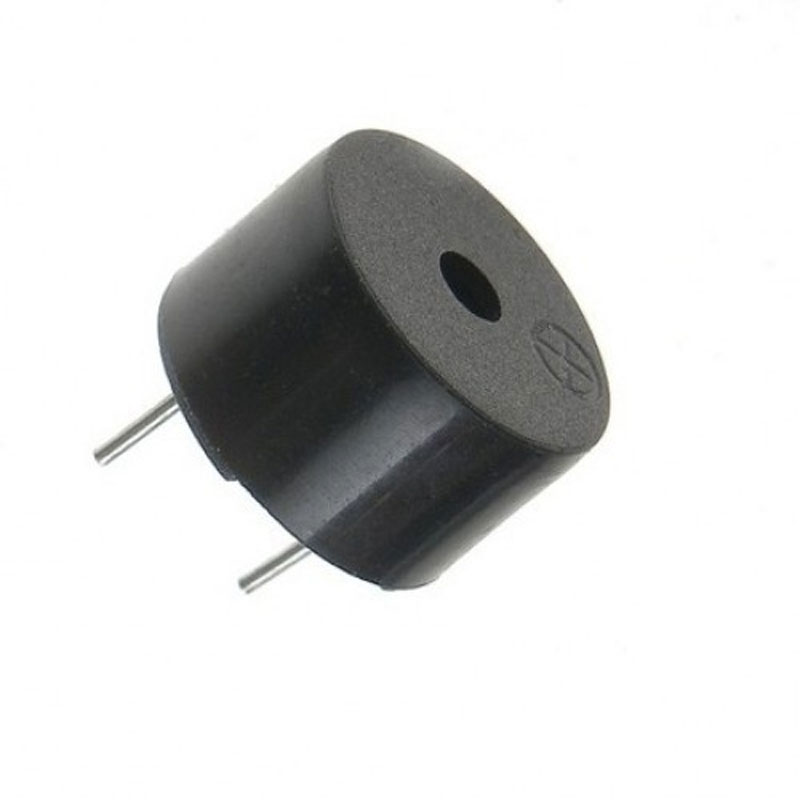
\includegraphics[width=7cm]{images/buzzer.jpg}
\caption*{Buzzer 5V}
\end{figure}
\subsubsection{How the system works}
The microcontroller receives commands from decoder MT8870, which decodes DTMF signals transmitted by user's mobile phone and control appliances following the commands. The system simultaneously get status of appliances and current date and time from real-time clock DS1307 to display to LCD.\\
Whenever the user is near the system, keypad is always available also.\\
The control signals will be sent to triac to lock/unlock current from power supply 220V to appliances.\\
Because main purposes of the system is remote control, notifying status of processing will be helped by the buzzer with different feedback signals.
\subsection{Software specification}
There's no a specific algorithm implemented in the program. The system continuously checks the DTMF signals sent by user's mobile phone to decide what tasks to perform.\\
Important functions which run in \textbf{main} function of the program will be described as below.
\begin{lstlisting}
void DocMatKhau() {
    char i;
    for (i = 0; i < 4; i++) Pas[i] = DSl3O7_Read(0x30 + i);
}
\end{lstlisting}
For saving memory purposes, the password is stored in DS1307 so that we read the it from DS1307 with pointer starting from \textcolor{blue}{0x30} to \textcolor{blue}{0x33}.
\begin{lstlisting}
void HienThoiGian() {
    // statements
}
\end{lstlisting}
Display current date and time base on data of real-time clock DS1307.
\begin{lstlisting}
void KiemTraMatKhau() {
    // statements
}
\end{lstlisting}
When user entering password to unlock the system, read input password and verify. The system will reject if password is invalid.
\begin{lstlisting}
void DieuKhienThietBi() {
    // statements
}
\end{lstlisting}
As the function name said, this one handles controlling appliances follow user's command.
\begin{lstlisting}
void HenGioTB1() {
    // statements
}

void HenGioTB2() {
    // statements
}
\end{lstlisting}
Set a specific time to automatically turn on/off appliances.
\begin{lstlisting}
void CaiMatKhau() {
    // statements
}
\end{lstlisting}
This function exists in case the user has demand on changing the password without touching the program inner the system. Note that, this cannot reset the password since authorization is needed in this process.
\begin{lstlisting}
void KiemTraTrangThaiThietBi() {
    LCD_Gotoxy(0, 1);
    if (TB1 == 1 && TB2 == 1) LCD_Puts("TB1:OFF  TB2:OFF");
    else if (TB1 == 1 && TB2 == 0) LCD_Puts("TB1:OFF   TB2:ON ");
    else if (TB1 == 0 && TB2 == 1) LCD_Puts("TB1:ON   TB2:OFF");
    else if (TB1 == 0 && TB2 == 0) LCD_Puts("TB1:ON   TB2:ON ");
}
\end{lstlisting}
Display status of appliances to LCD.
\begin{lstlisting}
void KiemTraThoiGianTuDong() {
    // statements
}
\end{lstlisting}
Automatic control task will be taken care of this function by checking current time and automatic setting time.
\begin{lstlisting}
void DieuKhienDTMF() {
    // statements
}
\end{lstlisting}
This function is called when DTMF process invoked. If-authenticated by entering correct password, the user have ability to control his appliances via his mobile phone.\\
Interrupts is also utilized, there are three interrupt functions to develop program that are  timer 0, timer 1 and external 1 interrupt.\\
Below are the details how interrupt functions constructed.
\begin{lstlisting}
void Timer0() interrupt TF0_VECTOR {
    TR0 = 0;
    // 50 ms
    TH0 = 0X3C;
    TL0 = 0XB0;
    dem1++;
    // 1 second
    if (dem1 == 20) {
        dem1 = 0;
        dem2++;
        // 120 seconds = 2 minutes
        if (dem2 == 120) {
            dem1 = dem2 = 0;
            TimeOut = 1;
            lock = 1;
        }
    }
    if (TimeOut == 0) TR0 = 1;
}
\end{lstlisting}
\newpage
\begin{lstlisting}
void Timer1() interrupt TF1_VECTOR {
    TR1 = 0;
    // 50 ms
    TH1 = 0X3C;
    TL1 = 0XB0;
    key = get_key();
    if (key == 13) {
        // unlock button pressed
        if (lock == 0) {
            lock = 1;
            bip(); bip(); bip();
        } else {
            bip();
            KtLock = 1;
            dem1 = dem2 = 0;
            TimeOut = 0;
            // send time out signal by turning on timer 0
            TR0 = 1;	
        }
    } else if (key == 12) {
        // menu button pressed
        bip();
        MODE = 1;
        dem1 = dem2 = 0;
        TimeOut = 0;
        TR0 = 1;
    }
    TR1 = 1;
}

void NgatNgoai1() interrupt 2 {
    bip();
    delay_ms(100);
    bip();
    delay_ms(100);
    bip();
    DTMF = 1;
    while (STD == 0);
    MODE = 0;
    dem1 = dem2 = 0;
    TimeOut = 0;
    TR0 = 1;                                                                    
}
\end{lstlisting}
Timer 0 handles time out process, make sure any process will last only 2 minutes for security purposes while timer 1 takes care of \textbf{menu} and \textbf{lock/unlock} button down event.\\
When DTMF signals come, the other interrupt that is external 1 will be invoked by set variable $\text{DTMF} = 1$.\\\\
If you have a need to learn more about how the program developed, go visit our repository uploaded to \href{https://github.com/trungnguyendx/Remote-Control-by-DTMF}{github.com/trungnguyendx/Remote-Control-by-DTMF}
\subsection{Test specification}
Devices for testing are voltage meter, light bulb and contacter. Circuit board prototype is built on PCB.\\
The testing process goes through following process:
\begin{itemize}
    \item Testing 5V power supply.
    \item Testing LCD, keypad interface.
    \item Testing communication between real-time clock, IC decoder and microcontroller.
    \item Testing excusetion block.
    \item Testing the whole system.
\end{itemize}

\newpage
%%%%%%%%%%%%%%%%%%%%%%%%%%%%%%%%%
\section{Design issues}\label{model}
These issues are problems make our solution difficult to design.
\subsection{Constraint issues}
As mentioned in \textbf{\nameref{introduction}}, our solution is the cheapest so that cost we have to minimize matters a lot and finally it comes to less than \$25 with a long life cycle is estimated to be 5 years.\\
Security is obviously a tough issue for all system and so our system is. We've considered a lot to decide password validation as security solution.\\
We use DTMF as the solution so the system needs to be located in places where there is phone coverage. Fortunately, in Vietnam, the coverage area is quite widely covered.\\
Since this is a signal remote control system and does not have a voice feedback system, it may be difficult for some users who is not familiar with technology.
\subsection{Functional issues}
The phone call can be made by breaker so that security is needed to detect the right user.\\
Input password process should be expired after amount of time. We've considered in detail and decided to set 2 minutes.\\
Simultaneous switching loaders that have high power may cause overcurrent at a time. Therefore, it should to be turned on one by one.\\
There should be different audio notification signals when controlling via mobile phone because the monitor cannot be seen.

\newpage
%%%%%%%%%%%%%%%%%%%%%%%%%%%%%%%%%
\section{Implementation}\label{eval}
\subsection{Schematics design}
\begin{figure}[h!]
\centering
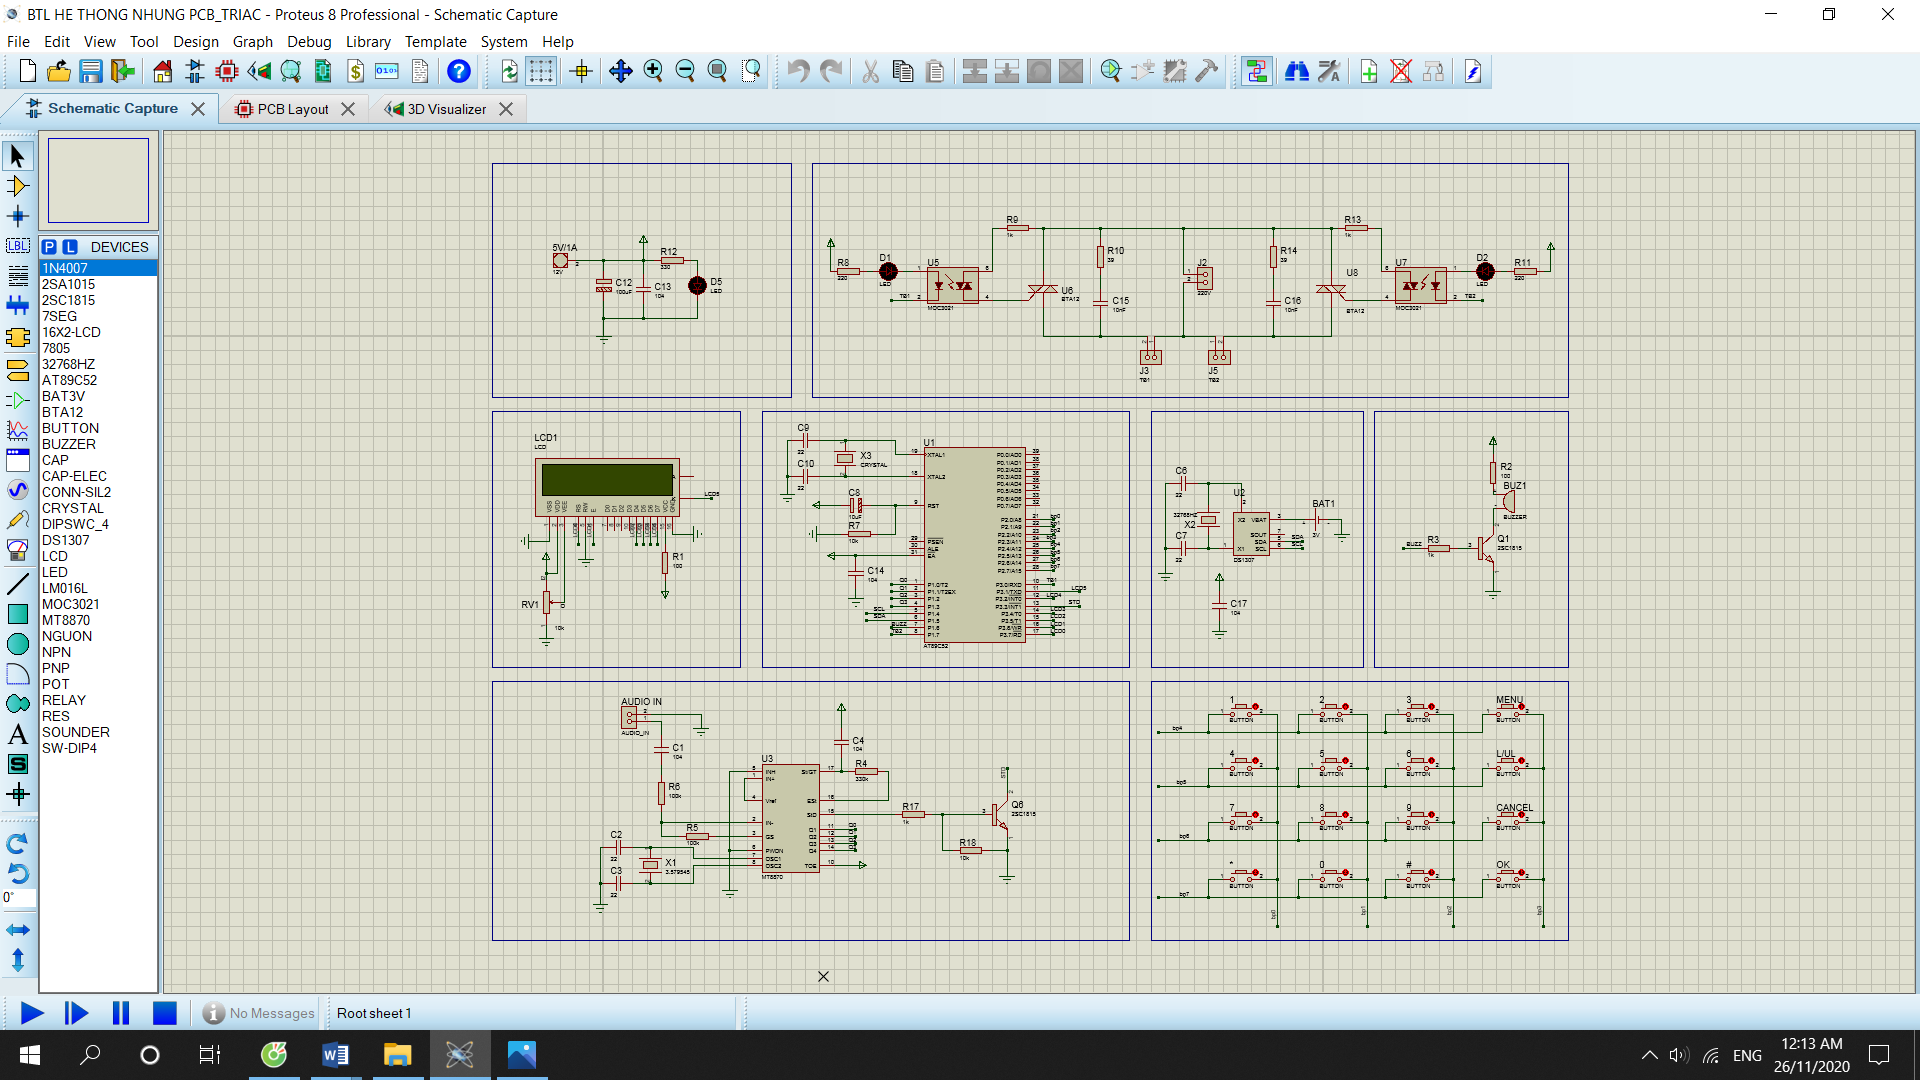
\includegraphics[width=17cm]{images/SCHE.PNG}
\caption*{Schematic}
\end{figure}
\noindent
Here is the schematic after the design is complete, we will go into details of each block to have a deeper look at them.
\subsubsection{Source}
The 5VDC power supply is taken from the 5V1A Adapter supplied for the active circuit. Capacitors C12 and C13 have the effect of filtering sources and noise pulses before supplying to the circuit. LED D5 is used to indicate power.
\begin{figure}[h!]
\centering
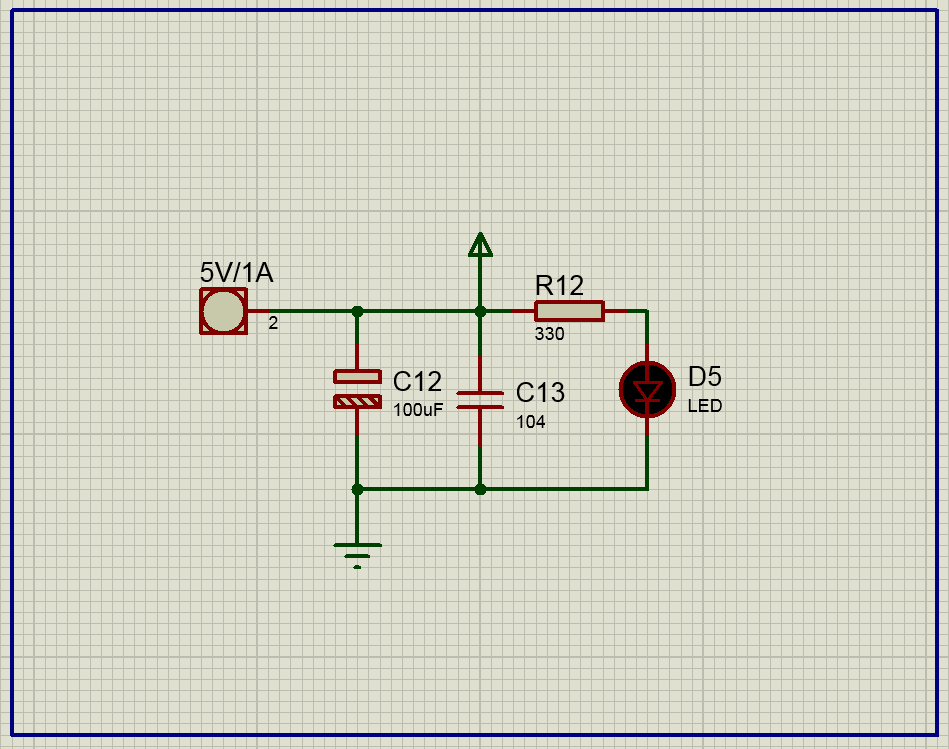
\includegraphics[width=10cm]{images/source.png}
\caption*{Source block schematic}
\end{figure}
\subsubsection{Central processing}
Including AT89S52 microcontroller and related circuits. Capacitor C8 and resistor R7 form a reset circuit at the power supply. X3 12MHz quartz and capacitors C9, C10 form the pulse level oscillator circuit for the microcontroller to operate. Capacitor C14 filters noise at the source of the microcontroller to avoid source noise which can make chip hang.\\
The pins are used as follows:
\begin{itemize}
    \item P1.0 - P1.3: Output of DTMF decoder. These are the pins contain data after decoding.
    \item P1.4 \& P1.5: Establish a connection between I2C and DS1307.
    \item P1.6: Control the buzzer
    \item P1.7: Control the II appliance.
    \item P2.0 - P2.7: Serving keypad scanning.
    \item P3.0: Control the I appliance.
    \item P3.1 \& P3.2: Generating signals to control LCD (control bus).
    \item P3.3: Connected to a DTMF decoder. When the user press a key on the his phone keypad to send a DTMF signal, this pin switches logic level from 1 to 0 to create an interrupt for the microcontroller.
    \item P3.4 - P3.7: Generating signals to control LCD (data bus).
\end{itemize}
\begin{figure}[h!]
\centering
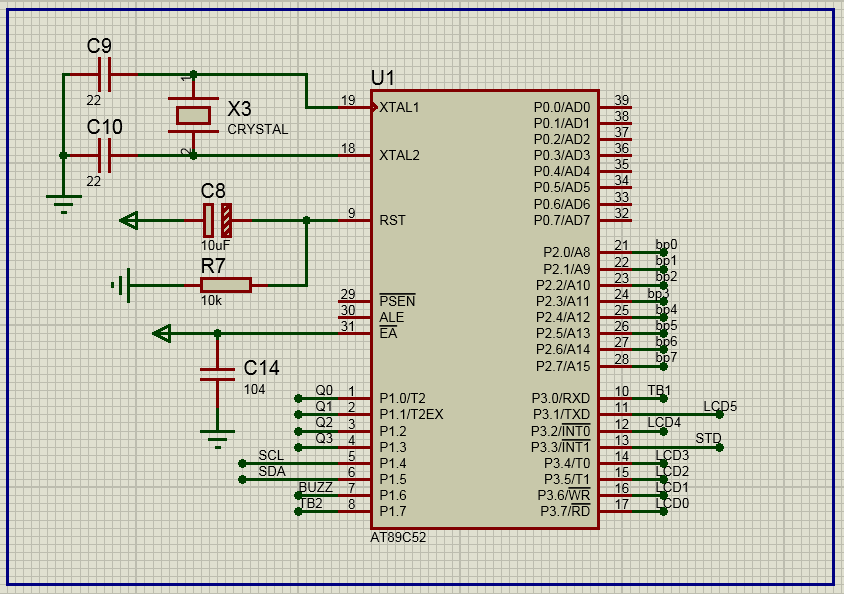
\includegraphics[width=15cm]{images/CP.PNG}
\caption*{Central processing block schematic}
\end{figure}
\subsubsection{Real-time clock}
Including real-time IC DS1307 and related components. 3v CMOS battery helps the IC to work even during power outages. The Quartz X2 32.768KHz provides the standard clock speed for the timer. Capacitor C17 filters source noise for the IC. Besides providing time, RAM of DS1307 is also used to save the password, time to automatically turn on and off devices. Communicate with the microcontroller via standard I2C.
\begin{figure}[h!]
\centering
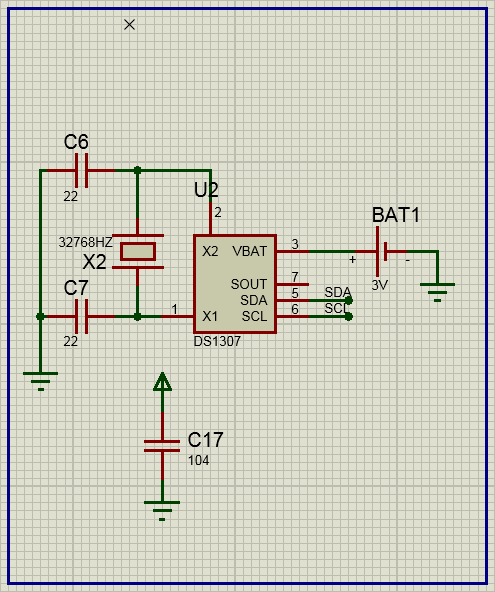
\includegraphics[width=10cm]{images/RTC.PNG}
\caption*{Real-time clock block schematic}
\end{figure}
\subsubsection{DTMF decoder}
Use IC MT8870 to decode DTMF signal from phone. Audio IN input is connected to the phone headset, output Q1-Q4 is connected to the microcontroller. The STD output is connected to transistor Q6 which acts as a NOT gate, connected to the microcontroller's breaker to confirm whether the phone key is pressed.
\begin{figure}[h!]
\centering
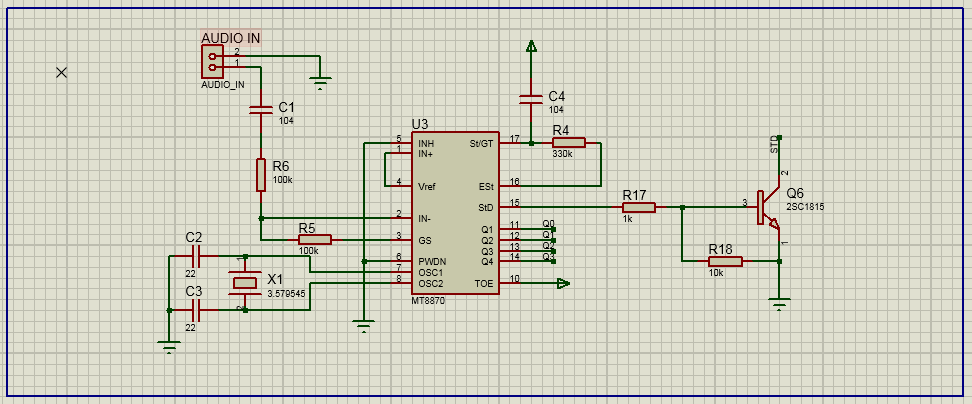
\includegraphics[width=17cm]{images/DTMF.PNG}
\caption*{DTMF block schematic}
\end{figure}
\subsubsection{Keypad 16}
Sixteen keys are connected in the form of a key matrix. Use key scanning to locate the pressed key. Consists of 12 keys as on the phone keypad and 4 function keys OK, CANCEL, LOCK / UNLOCK, MENU.
\begin{figure}[h!]
\centering
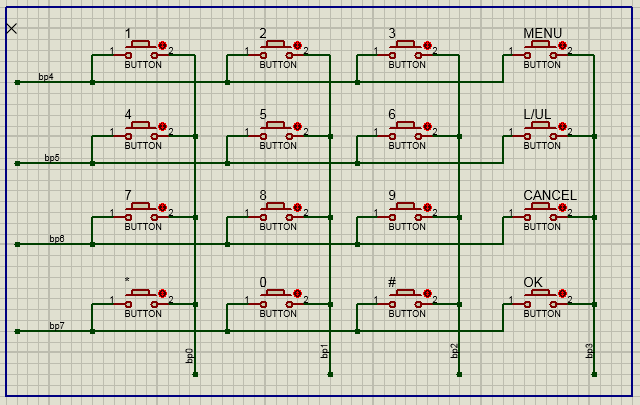
\includegraphics[width=13cm]{images/keypad.PNG}
\caption*{Keypad block schematic}
\end{figure}
\subsubsection{Audio notification}
Passive Buzzer (Buzzer emits a variable frequency, based on the frequency of control) and 1 transistor to control. The buzzer will emit a sound depending on the control signal, which has the effect of notifying the keys that have been pressed or the status of the appliances (for the DTMF remote control since the LCD cannot be observed).
\begin{figure}[h!]
\centering
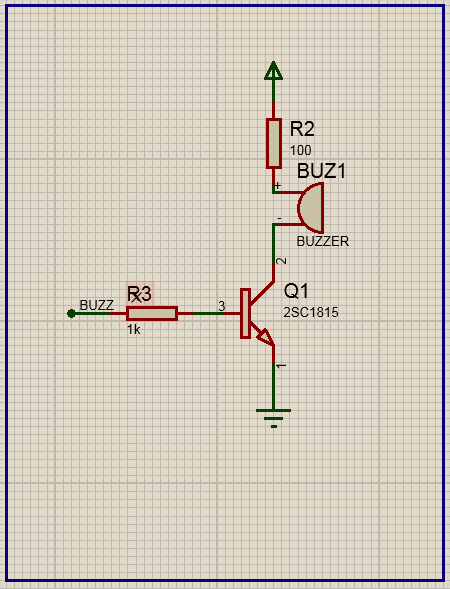
\includegraphics[width=7cm]{images/audio.PNG}
\caption*{Audio notification block schematic}
\end{figure}
\subsubsection{Power}
Consists of 2 triac BTA12 combined with 2 opto triac MOC3021 to control two 220v appliances. When there is signal from the microcontroller, the opto triac triggers the triac to work. On the 2 poles of each triac there is a snubber circuit to prevent transformers on the T1 and T2 pins to avoid self-conducting triac.
\begin{figure}[h!]
\centering
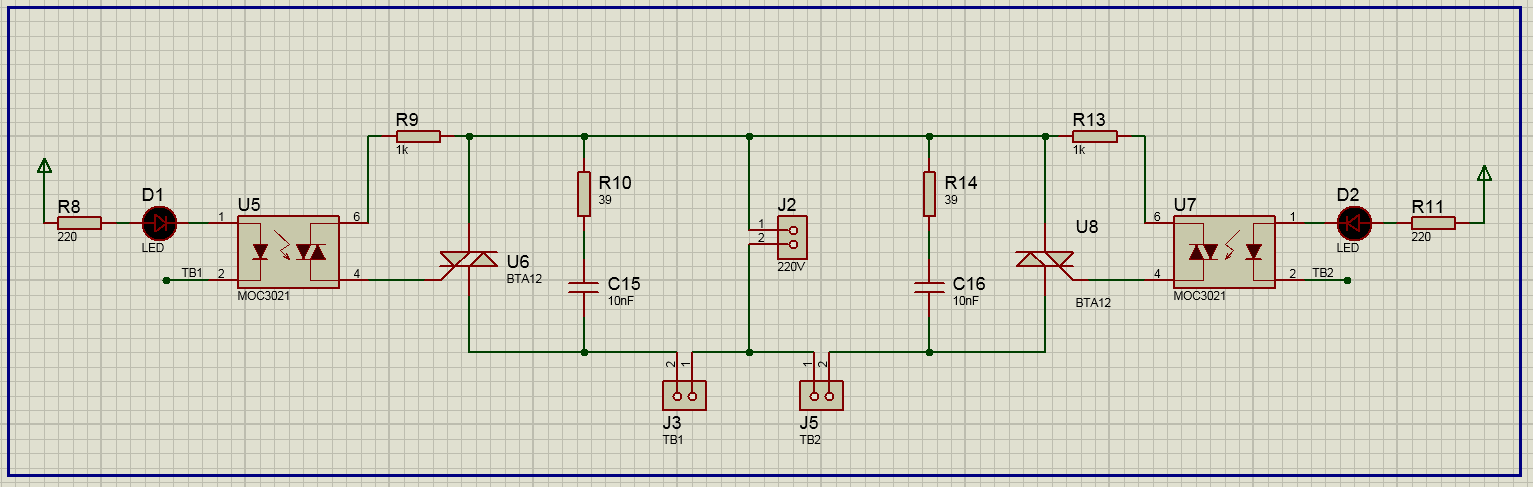
\includegraphics[width=17cm]{images/power.png}
\caption*{Power block schematic}
\end{figure}
\subsubsection{Display}
Using a 16x2 LCD communicates with the microcontroller via 4bit mode (using only 4 data pins from the D4-D7). For contrast, it is adjusted by variable resistor RV1.
\begin{figure}[h!]
\centering
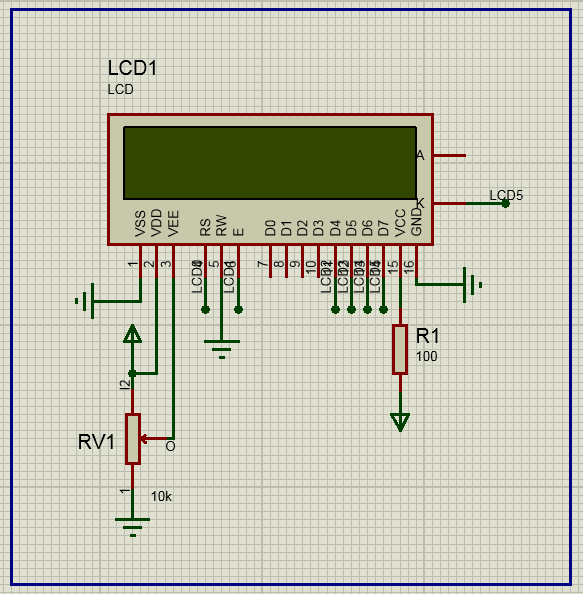
\includegraphics[width=12.5cm]{images/display.PNG}
\caption*{Display block schematic}
\end{figure}

\subsection{Circuit visualization}
After designing the schematics on Proteus, we proceed to put our circuit in 3D simulation.
\begin{figure}[h!]
\centering
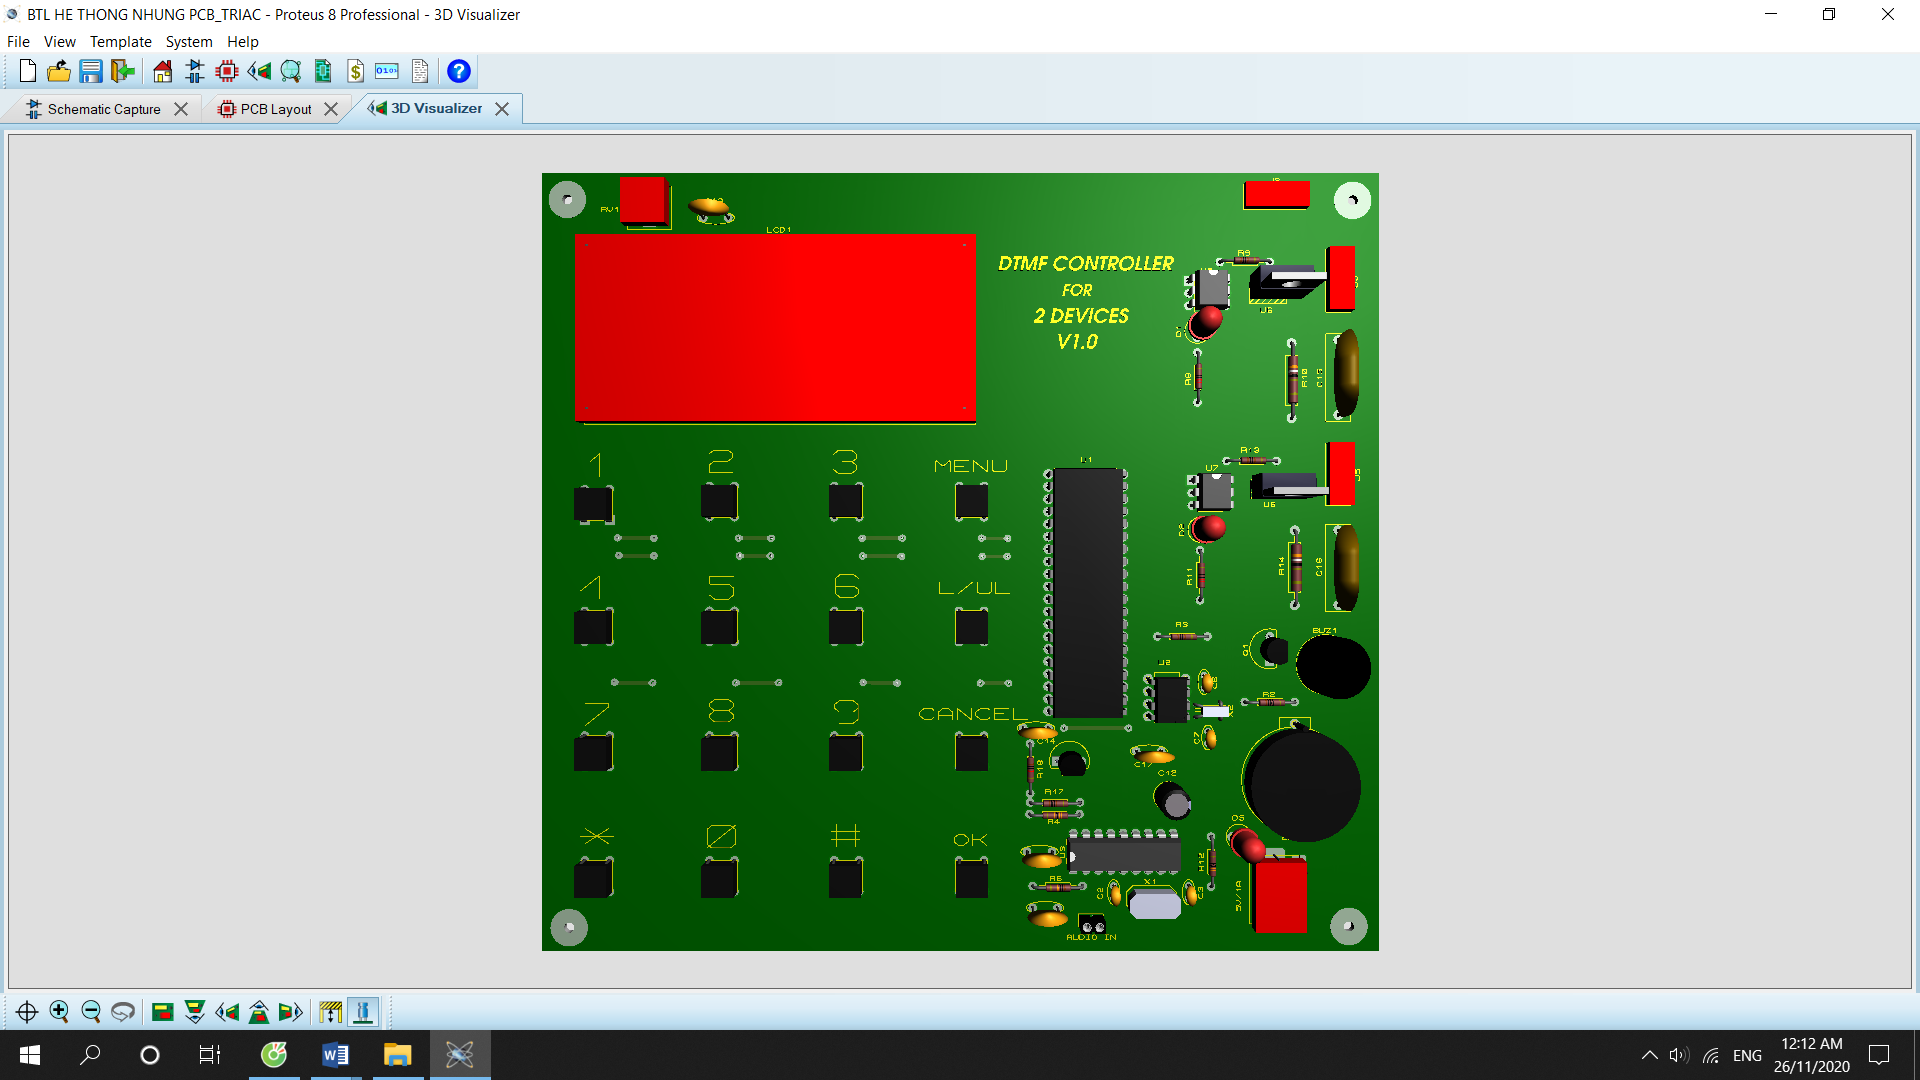
\includegraphics[width=17cm]{images/3d.PNG}
\caption*{3D visualization}
\end{figure}\\
The prototype was not on breadboard, but the PCB.
\begin{figure}[h!]
\centering
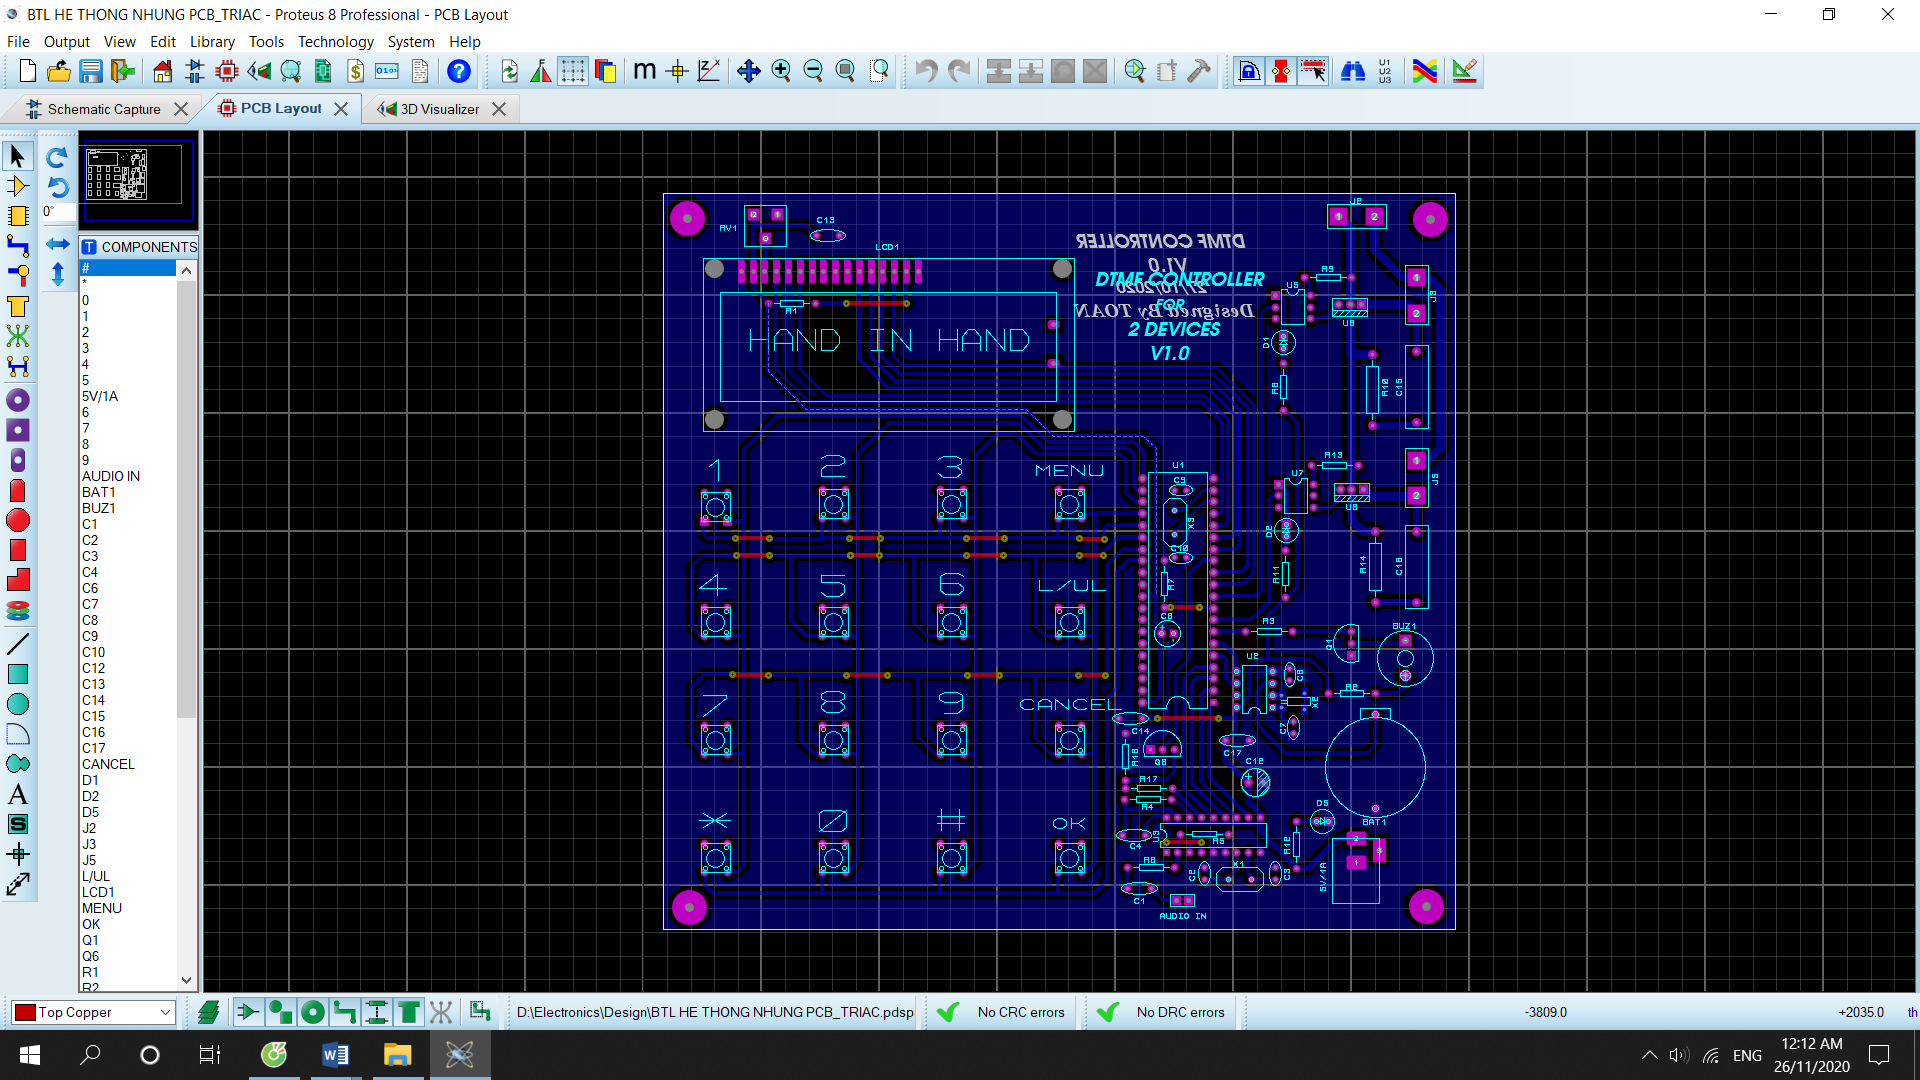
\includegraphics[width=17cm]{images/PCB.PNG}
\caption*{PCB layout}
\end{figure}
\subsection{Hardware deployment}
After visualization, we see no problem then we go to make a printed circuit board.
\begin{figure}[h!]
\centering
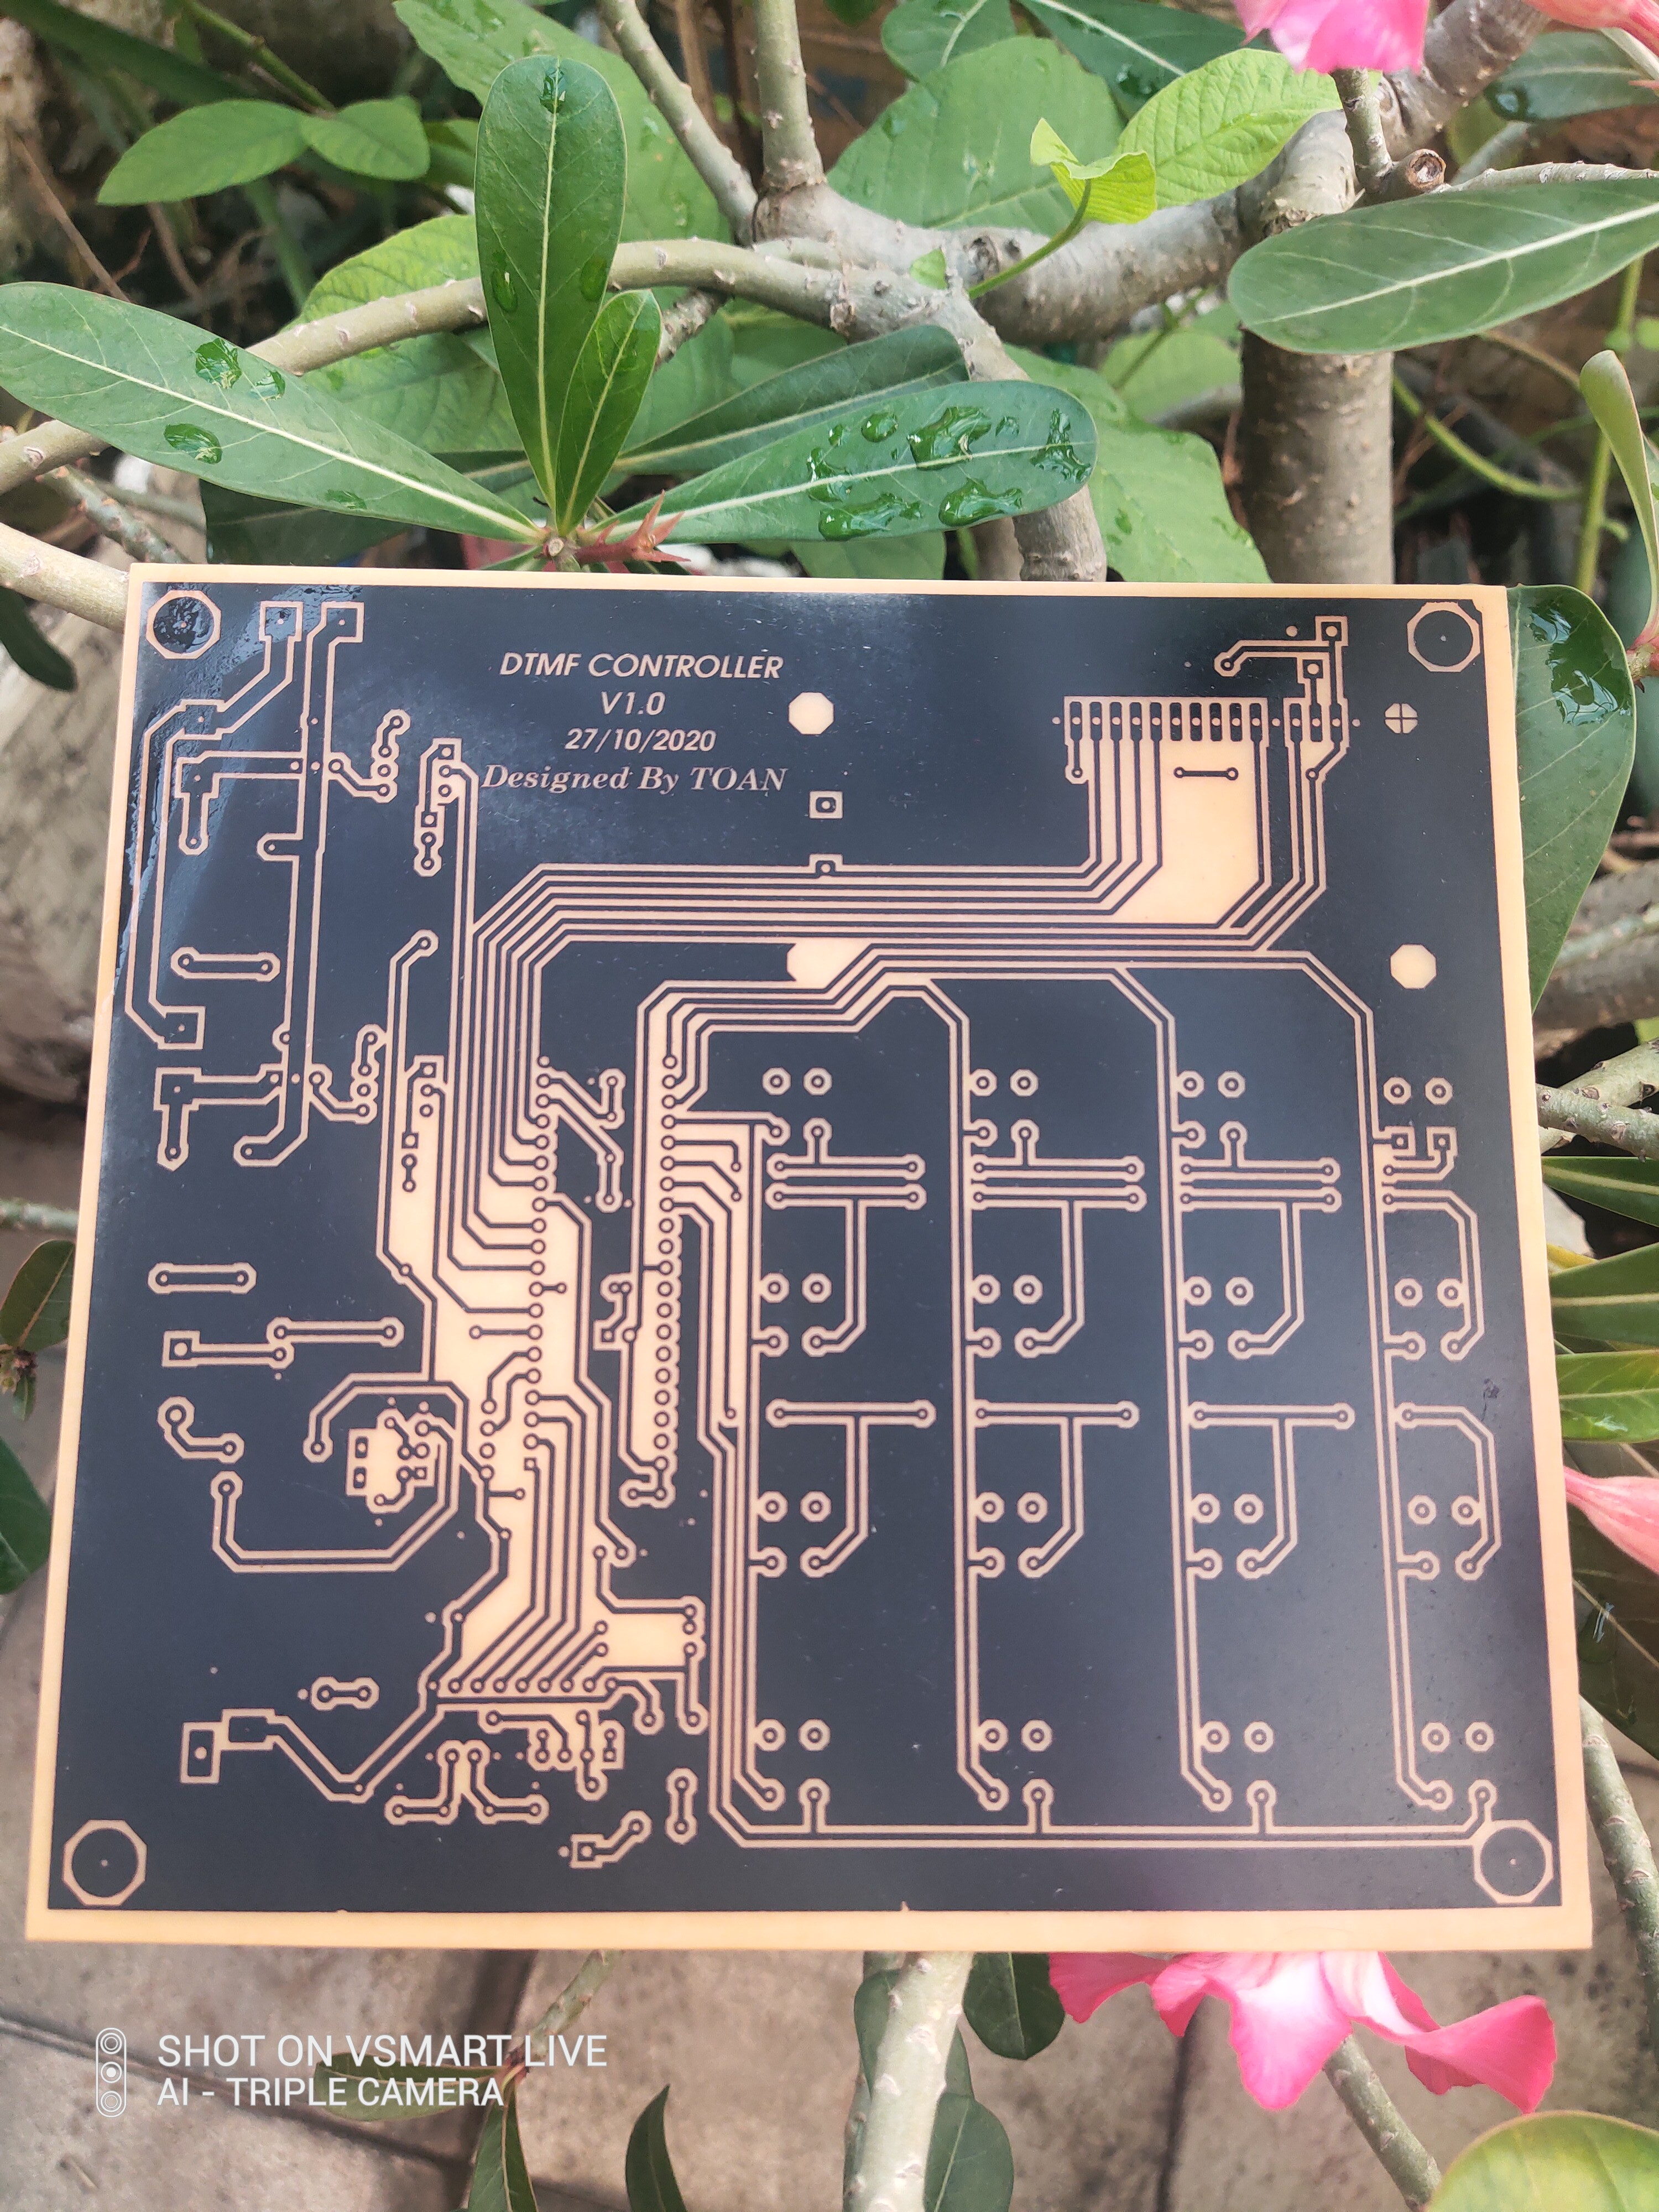
\includegraphics[width=8.2cm]{images/back.jpg}
\caption*{Back of the PCB}
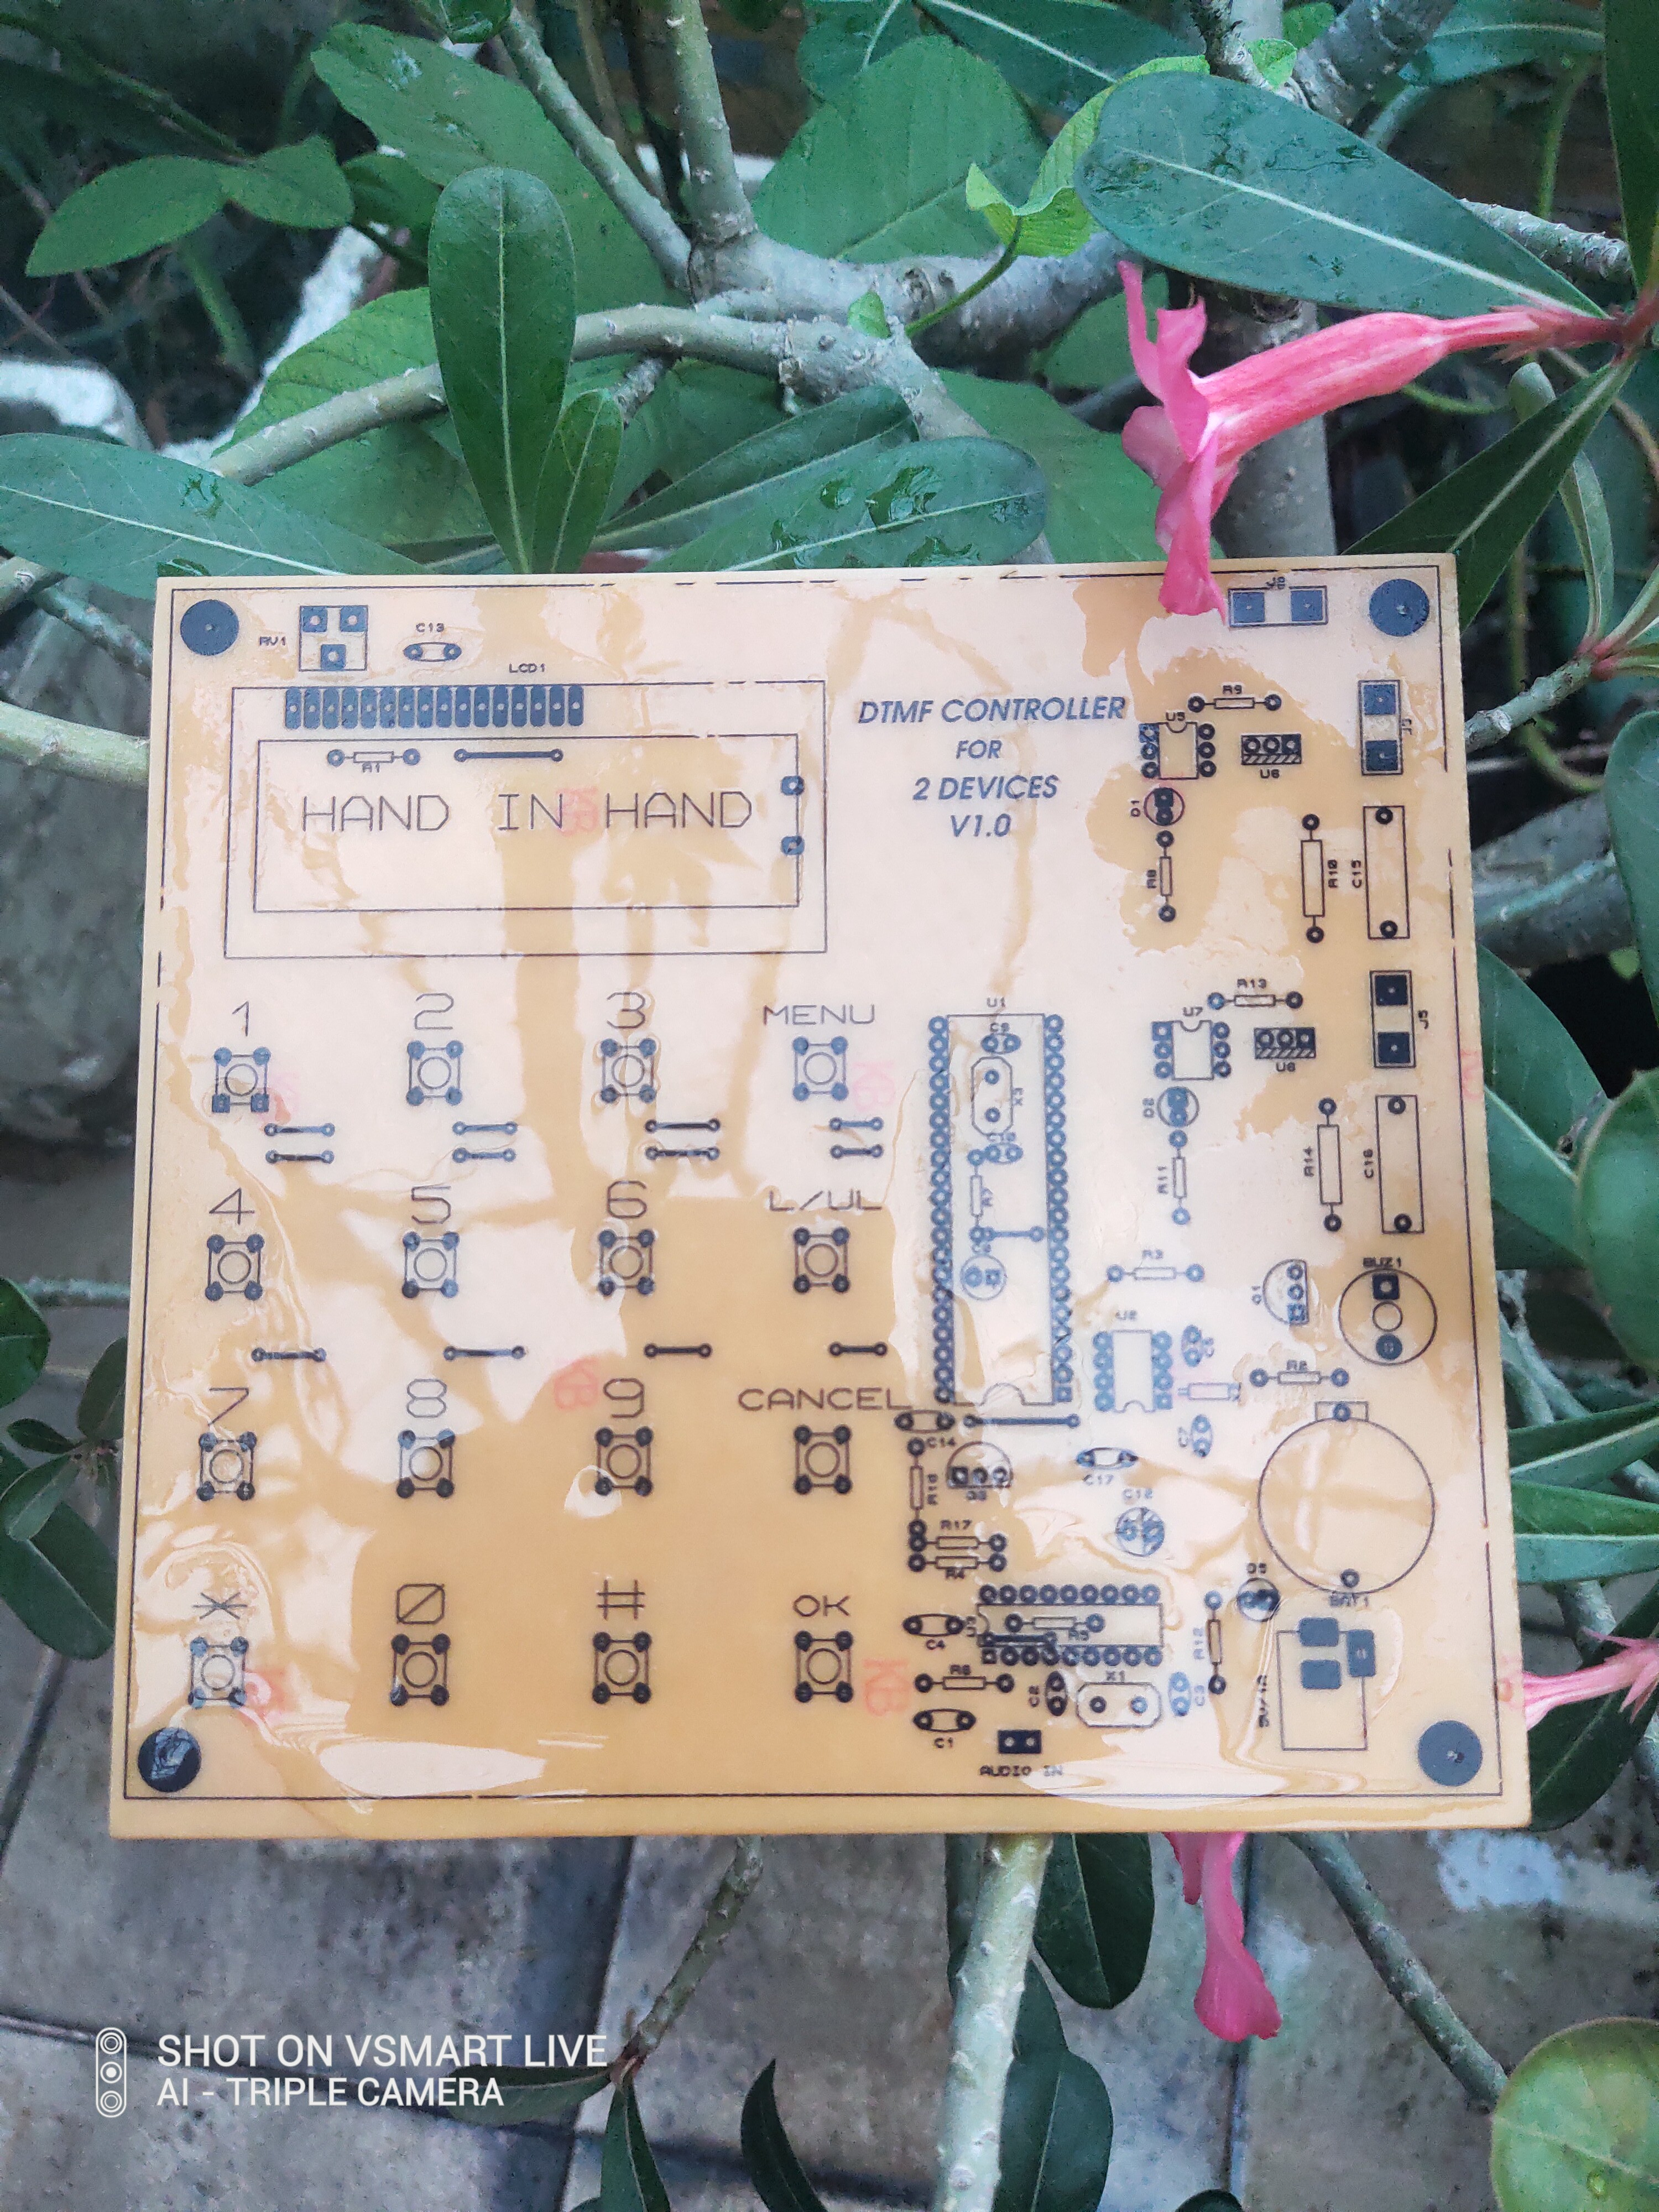
\includegraphics[width=8.2cm]{images/front.jpg}
\caption*{Front of the PCB}
\end{figure}
\newpage
\noindent
we are experienced in hardware implementation so the circuit development process does not take too long.
\begin{figure}[h!]
\centering
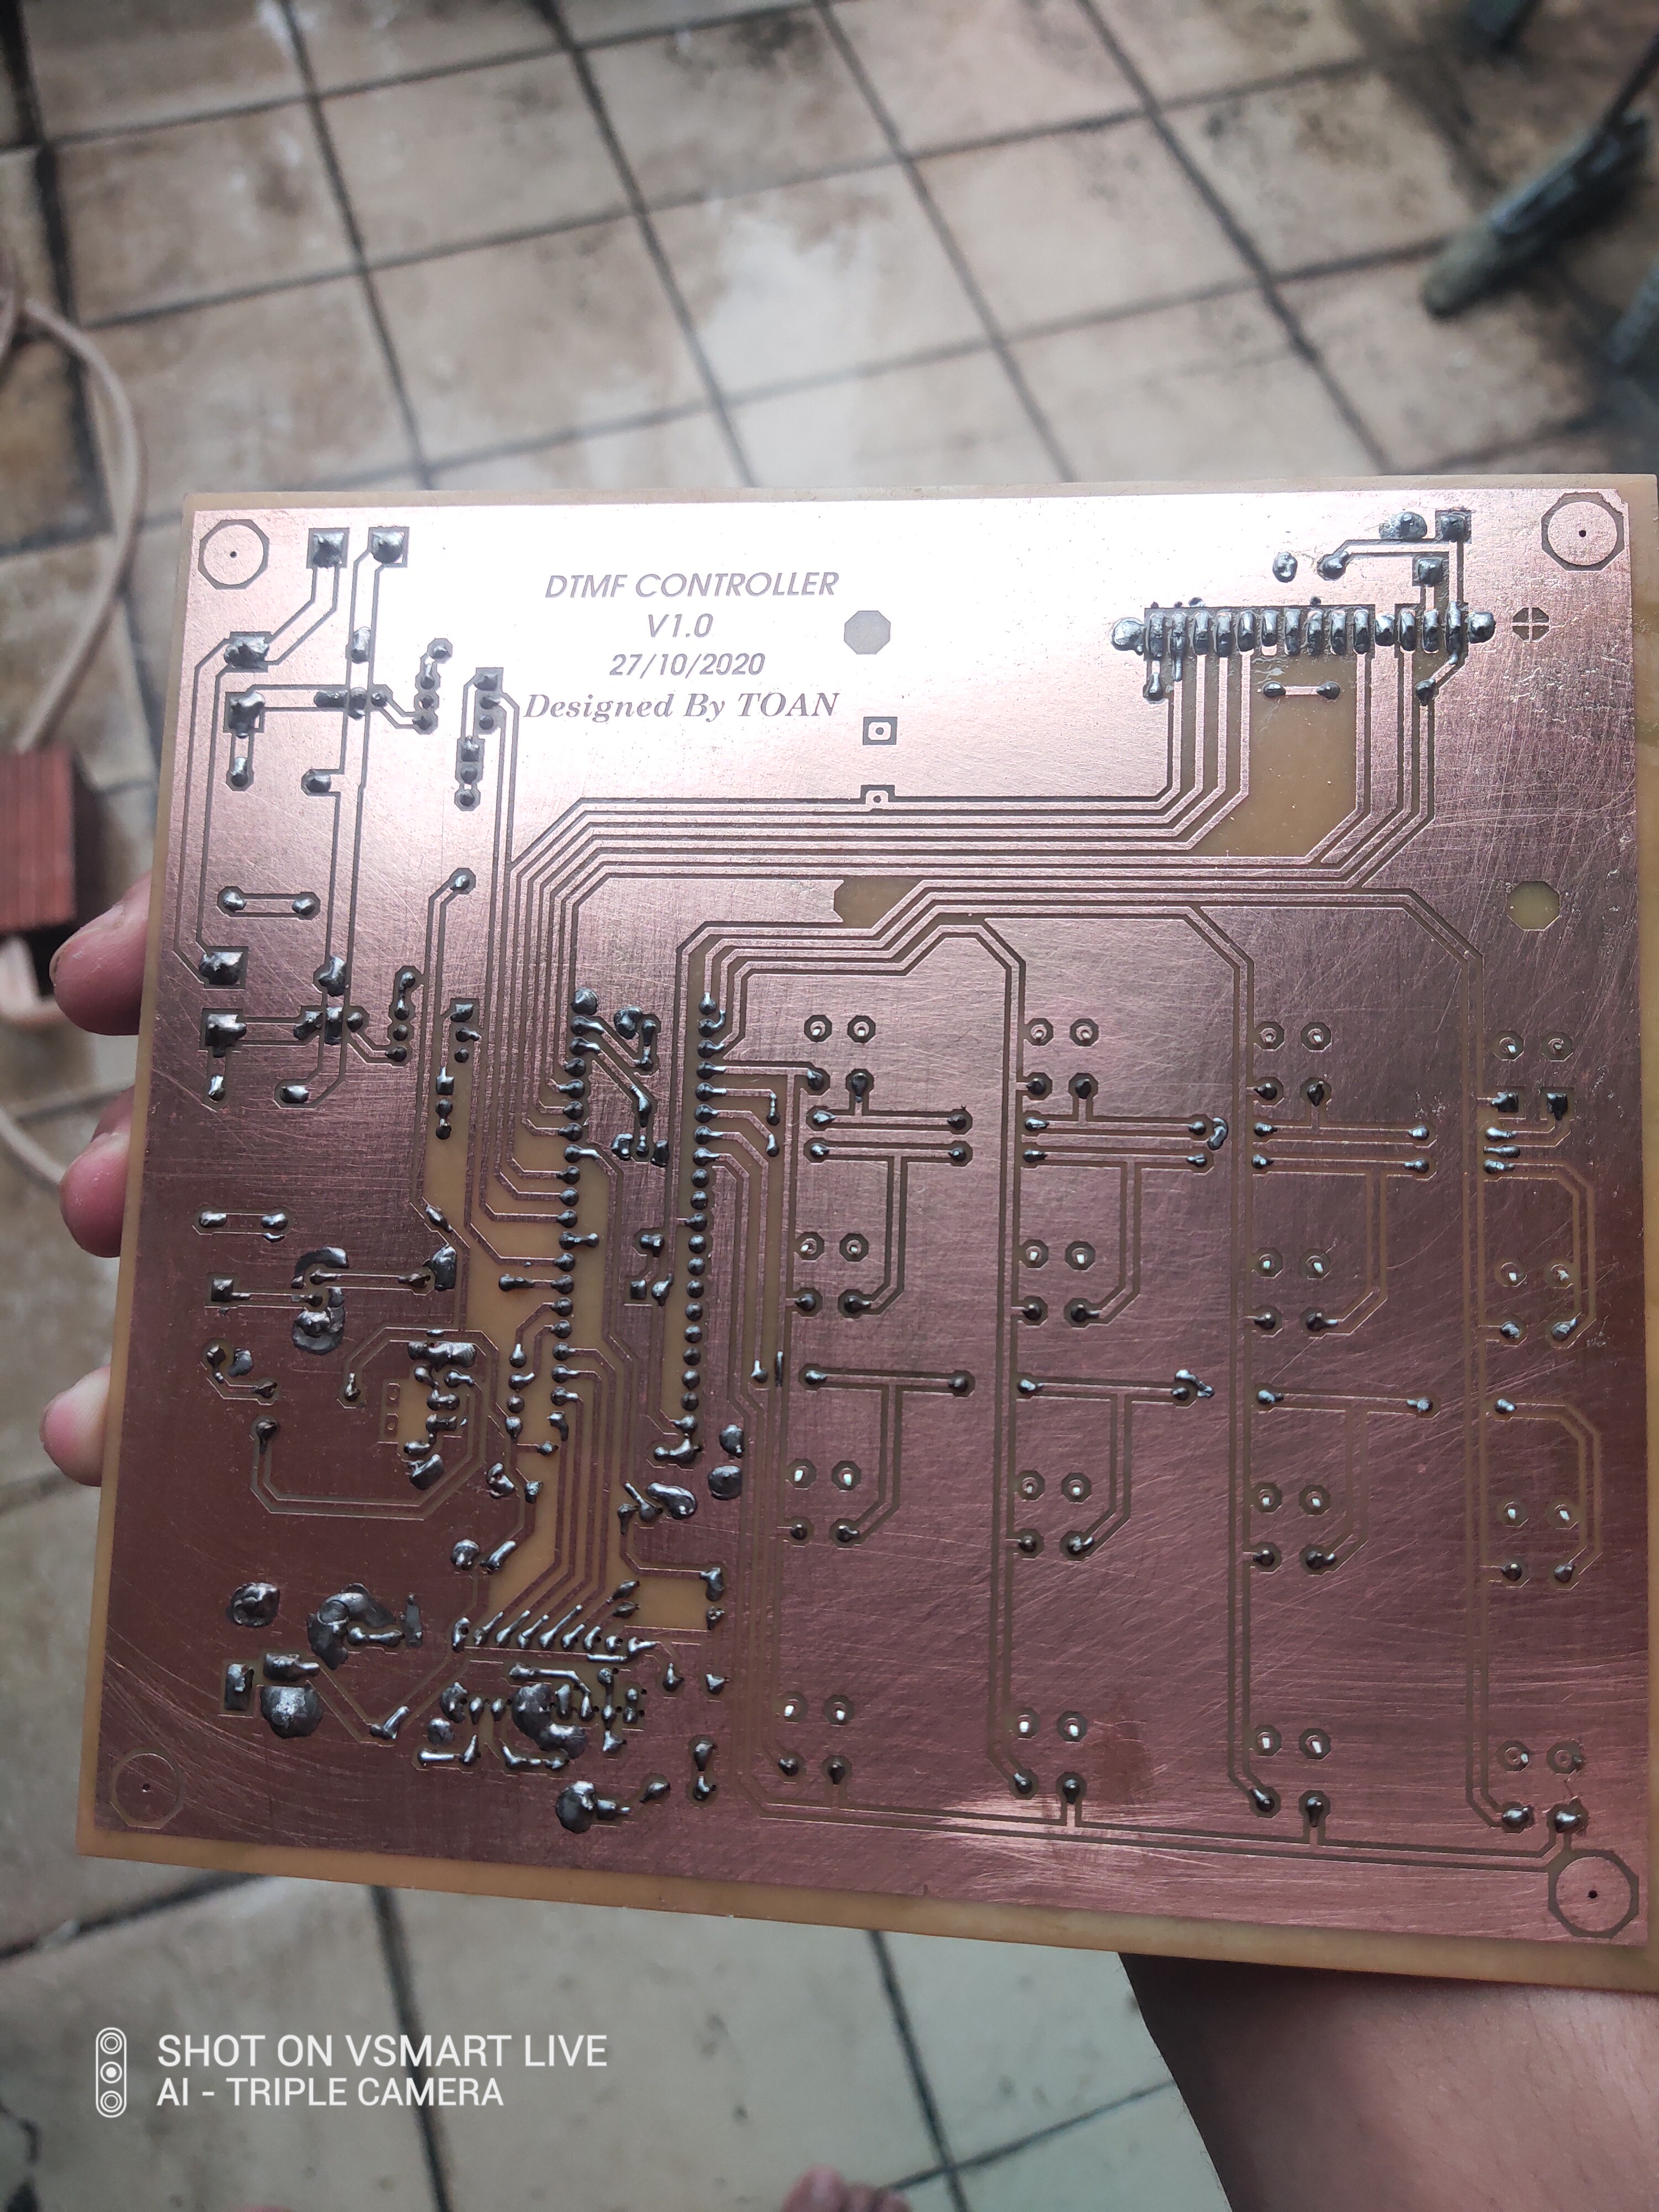
\includegraphics[width=9.5cm]{images/backk.jpg}
\caption*{Back of the circuit}
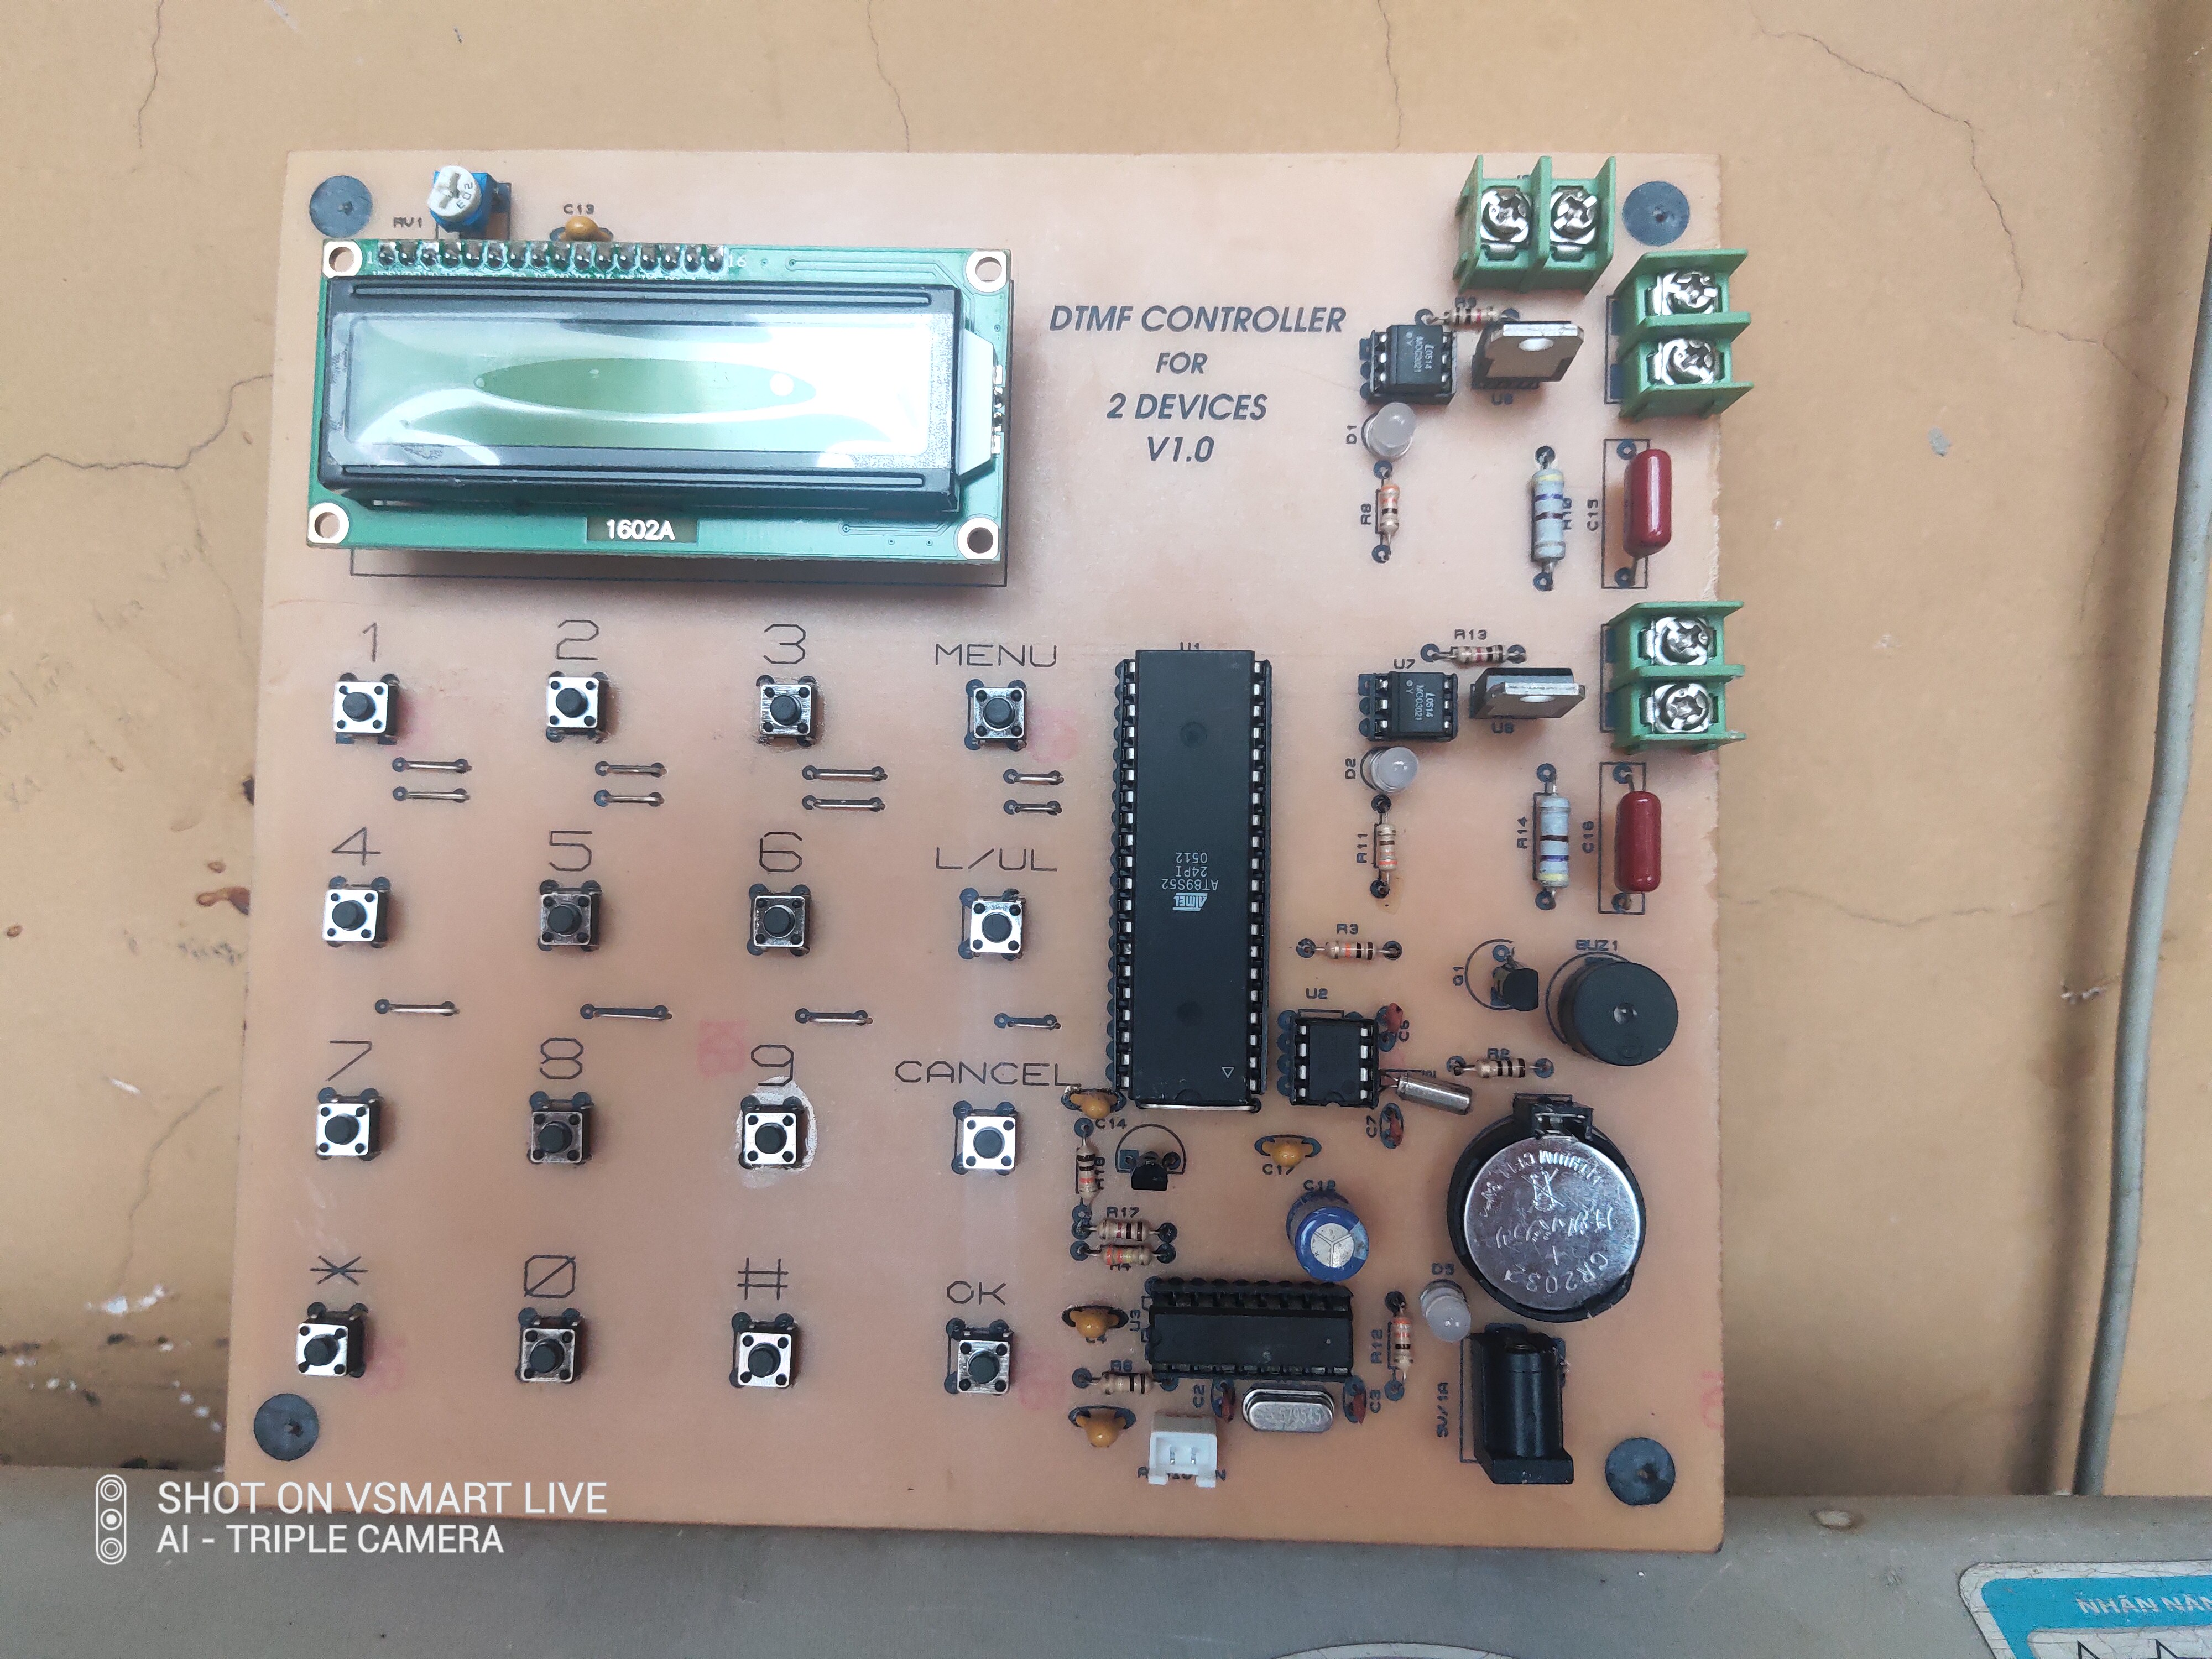
\includegraphics[width=13cm]{images/frontt.jpg}
\caption*{Front of the circuit}
\end{figure}
\newpage
\noindent
And here is our system.
\begin{figure}[h!]
\centering
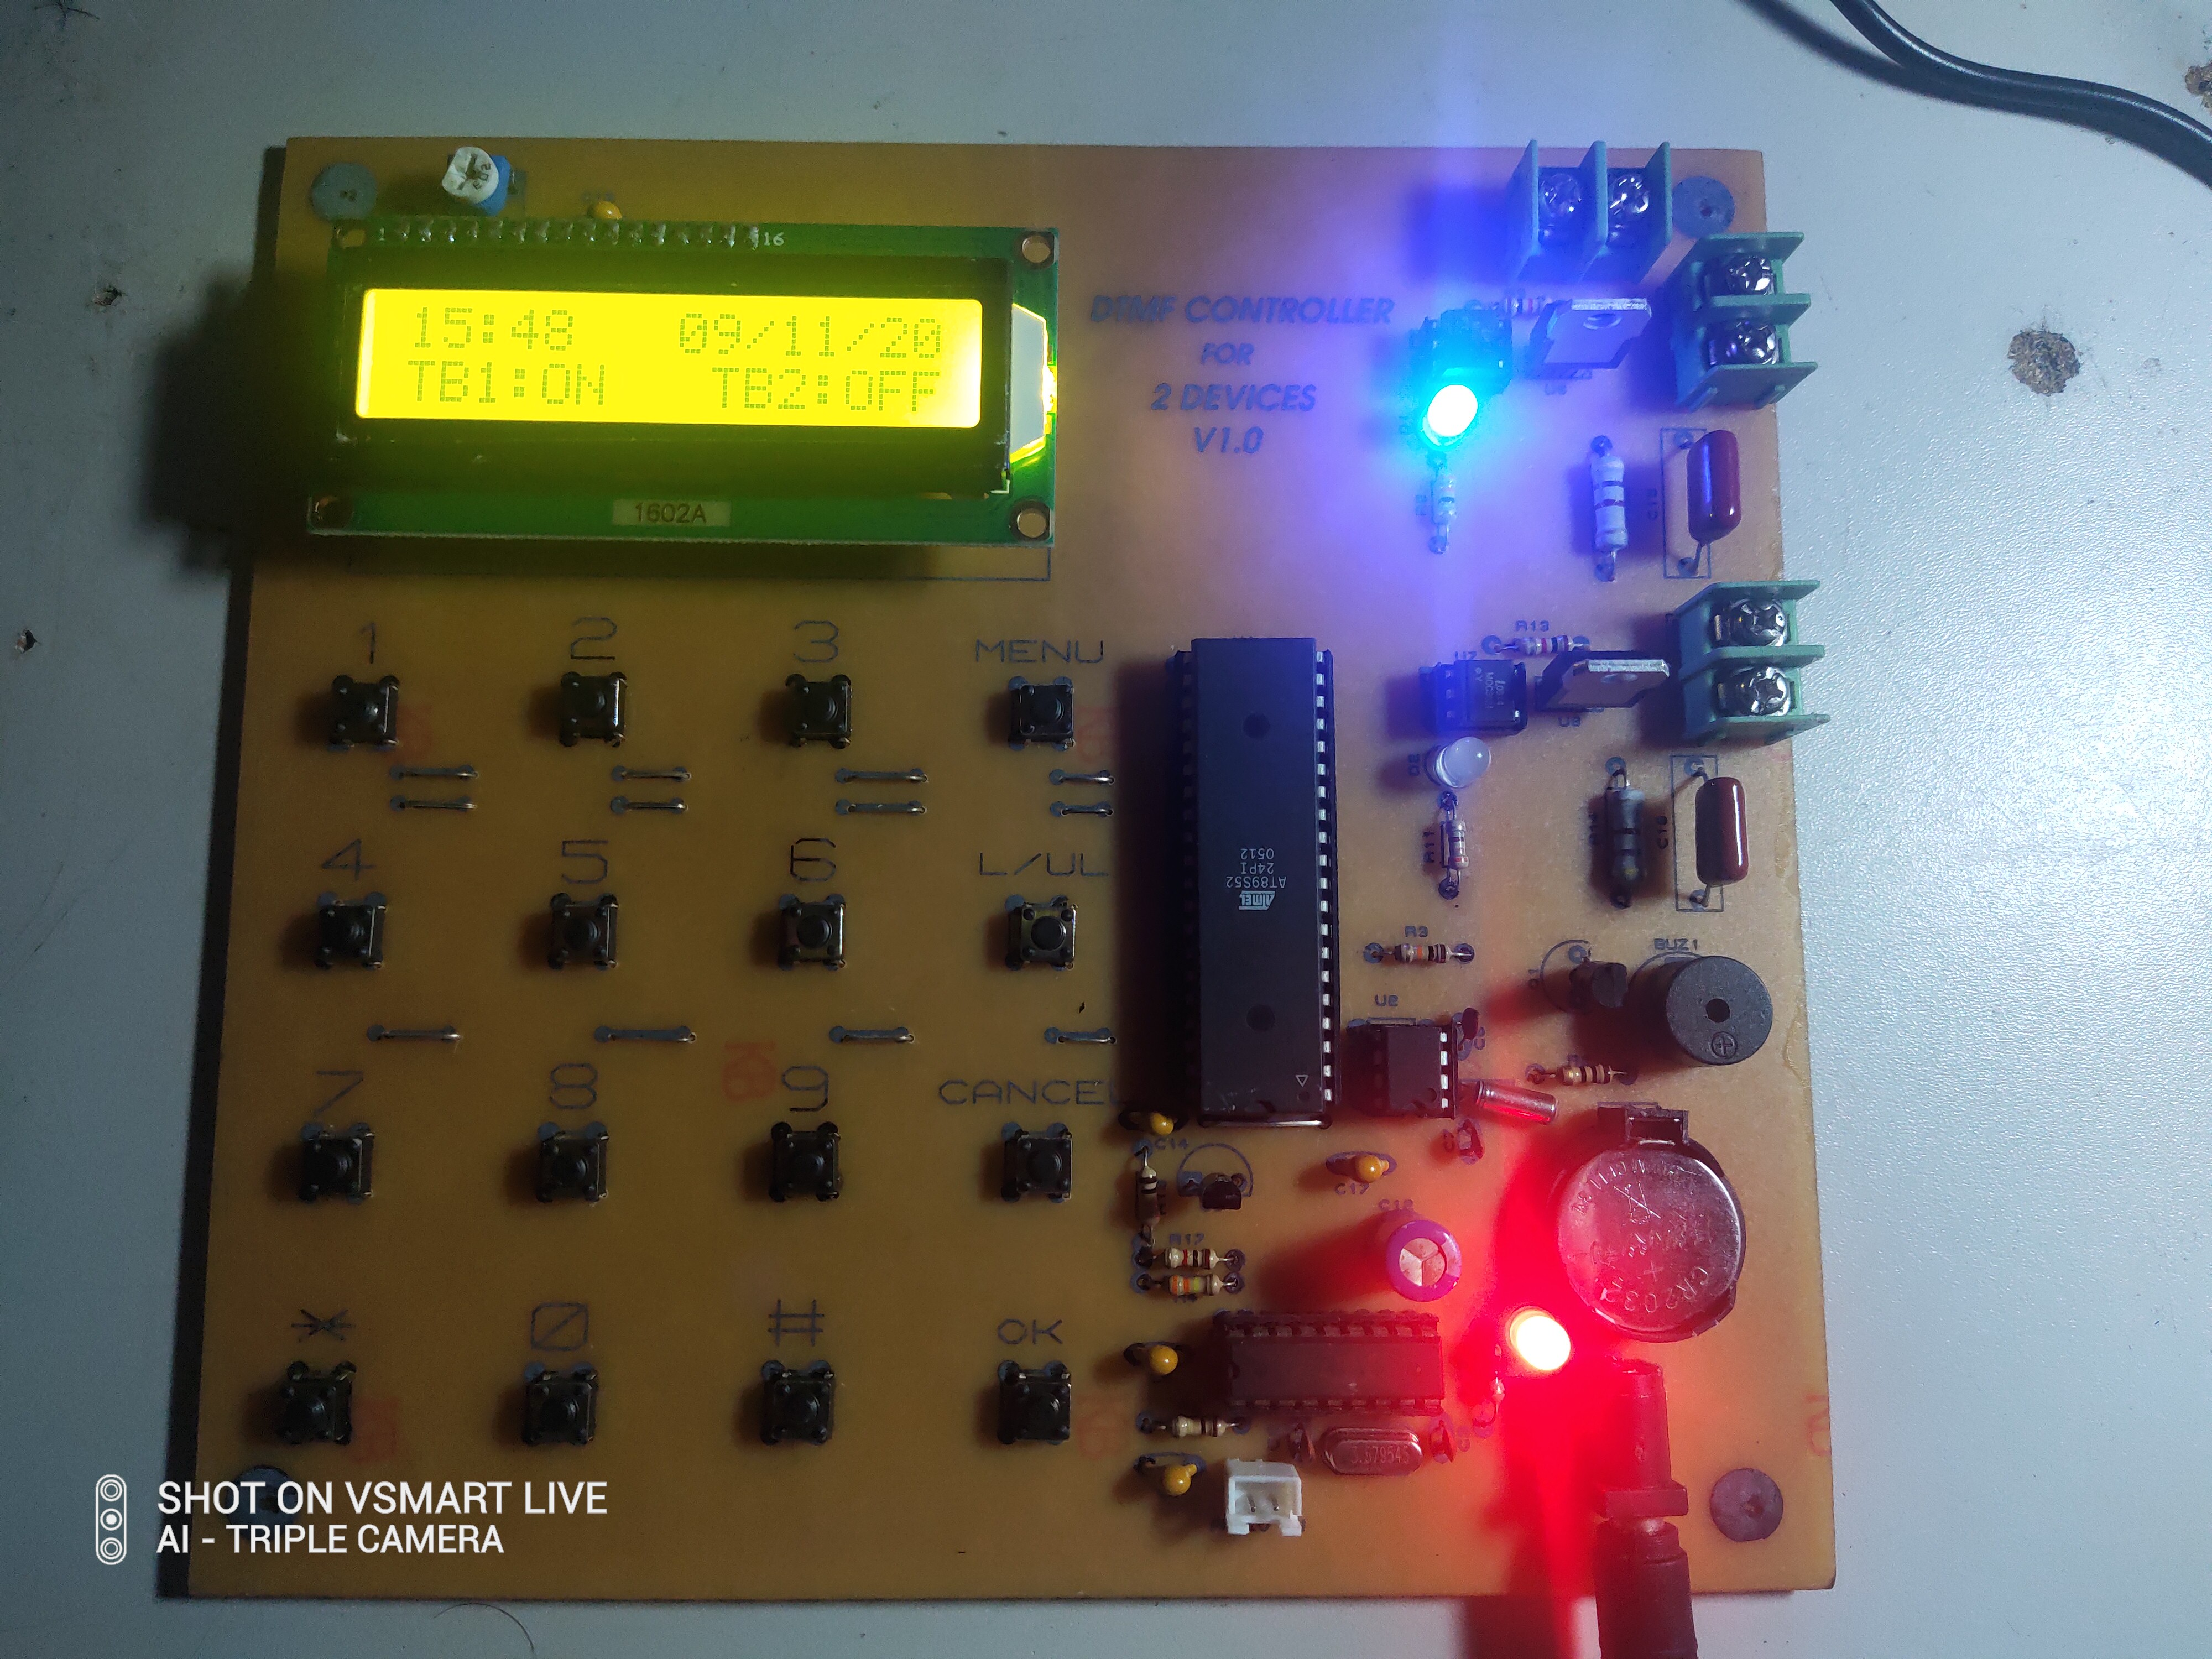
\includegraphics[width=17cm]{images/working.jpg}
\caption*{The system is working}
\end{figure}\\
The red LED is responsible for power notification, the LCD will display the time in the upper left corner and the date in the upper right corner.\\
For the status of appliances, it will be shown in the second row of the LCD. If you notice, you'll see that appliance I is on and there is one blue LED is on since the duty of notification will be taken over by the blue LEDs.\\
We run to the testing phase and find some software problems. However, it was also quickly corrected.
\newpage
%%%%%%%%%%%%%%%%%%%%%%%%%%%%%%%%%
\section{Conclusion}
\subsection{Advantages}
\begin{itemize}
    \item The circuit is easy to implement due to the AT89S52 we did learn in Microprocessor.
    \item The cost is minimized.
    \item The system is easy to use for most of people.
\end{itemize}
\subsection{Disadvantages}
\begin{itemize}
    \item Security is not strong since the password is short for quick access purposes.
    \item The system cannot detect the breakers if they're trying to get the access.
    \item The feedback is not intuitive as only audio signal for notification. This makes some user find difficult to use.
\end{itemize}
\subsection{Product development}
We intend to develop the product in some directions to make our product simpler and reach more people by
\begin{itemize}
    \item Preventing breakers from getting access thanks to some constraint in password input process.
    \item Modulating our circuit board for easy assembly and repair.
    \item Giving the system the ability to normally work without the need for a direct power supply.
    \item Providing voice feedback to help users out of some troubles.
    \item Not only allowing control appliances via DTMF signals, but bluetooth or wifi also.
\end{itemize}
\newpage
%%%%%%%%%%%%%%%%%%%%%%%%%%%%%%%%%
\begin{thebibliography}{80}


\bibitem{https://www.keil.com/dd/docs/datashts/atmel/at89s52_ds.pdf} KEIL.
``\textbf{www.keil.com/dd/docs/datashts/atmel/at89s52\_ds.pdf}''

\bibitem{https://components101.com/misc/4x4-keypad-module-pinout-configuration-features-datasheet} COMPONENTS101.
``\textbf{components101.com/misc/4x4-keypad-module-pinout-configuration-features-datasheet}''

\bibitem{https://components101.com/modules/mt8870-dtmf-decoder-module} COMPONENTS101.
``\textbf{components101.com/modules/mt8870-dtmf-decoder-module}''

\bibitem{https://datasheets.maximintegrated.com/en/ds/DS1307.pdf} maxim intergrated.
``\textbf{datasheets.maximintegrated.com/en/ds/DS1307.pdf}''

\bibitem{https://www.thingbits.in/products/standard-lcd-16x2-display} thingbits.
``\textbf{www.thingbits.in/products/standard-lcd-16x2-display}''

\bibitem{https://components101.com/ics/moc3021-triac-driven-optoisolator-pinout-equivalent-datasheet} COMPONENTS101.
``\textbf{components101.com/ics/moc3021-triac-driven-optoisolator-pinout-equivalent-datasheet}''

\bibitem{https://www.st.com/resource/en/datasheet/bta12.pdf} ST.
``\textbf{www.st.com/resource/en/datasheet/bta12.pdf}''

\bibitem{http://tinkbox.ph/sites/tinkbox.ph/files/downloads/5V_BUZZER_MODULE.pdf} TINKBOX.
``\textbf{tinkbox.ph/sites/tinkbox.ph/files/downloads/5V\_BUZZER\_MODULE.pdf}''

\end{thebibliography}
\end{document}

